\documentclass[10pt,a4paper]{report}
\usepackage{geometry}
%\usepackage[utf8]{inputenc} % Apprently not useful with LuaLaTeX
\usepackage[T1]{fontenc}
\usepackage[british]{babel}
\usepackage{amsmath} % mathematical symbols
\usepackage{amsfonts} % mathematical symbols
\usepackage{amssymb} % mathematical symbols
\usepackage{graphicx} % figures
\usepackage{array} % for new column type
\usepackage{tabu} % for custom line width in tables
\usepackage{longtable} % multi-page tables
\usepackage[table,xcdraw]{xcolor}
\usepackage{fancyhdr} % headers and footers
\usepackage{lastpage}	% total page count
\usepackage{float}
\usepackage{multirow}
\usepackage[bottom]{footmisc} % footnotes at the bottom of the page
\usepackage{subcaption} % subfigures
\usepackage{verbatim} % comment environment
\usepackage[backend=bibtex]{biblatex}
%\usepackage{bbding} % checkmark
\usepackage{pifont} % checkmark and cross
%\usepackage{nicematrix} % to fix colorcell overalpping borders
\usepackage{hhline} % partial hline for long division
\usepackage{minted} % python code highlight
\usepackage[minted,breakable]{tcolorbox} % minted title
\usepackage{csquotes} % localized quotes
\usepackage{caption} % caption for side by side fig and tab

\bibliography{db.bib}

%THIS NEEDS TO BE LOADED AFTER `longtable` TO PREVENT CONFLICTS
\usepackage{arydshln} % dashed lines in tables

\usepackage{fontspec} % custom font
\setmainfont{Ubuntu-R}[
  BoldFont        = Ubuntu-B,
  ItalicFont      = Ubuntu-RI,
  BoldItalicFont  = Ubuntu-BI
]
\setmonofont{UbuntuMono-R}[
  BoldFont        = UbuntuMono-B,
  ItalicFont      = UbuntuMono-RI,
  BoldItalicFont  = UbuntuMono-BI
]

\usepackage{hyperref}	% links
\hypersetup{
  pdftitle={Barcodes and QR-Codes},
  pdfauthor={Louis Heredero},
  colorlinks=true,
  linkcolor=black,
  citecolor=black,
  filecolor=black,
  urlcolor=blue
}

\pagestyle{fancy}
\setlength{\headheight}{15pt}

\renewcommand{\headrulewidth}{1pt}
\fancyhead[L]{\leftmark}
\fancyhead[C]{}
\fancyhead[R]{\rightmark}

\renewcommand{\footrulewidth}{1pt}
\fancyfoot[L]{Louis Heredero 5D}
\fancyfoot[C]{\thepage/\pageref{LastPage}}
\fancyfoot[R]{September 2022}

% Black cell for representing barcodes in tables
\newcommand*{\bbar}{\cellcolor{black}}
\newcolumntype{C}[1]{>{\centering\arraybackslash}p{#1}}

% Rotate table header
\newcommand{\rot}[1]{\hspace{5pt}\rotatebox{90}{#1\hspace{10pt}}\hspace{5pt}}

% Long division vertical bar
\newcommand{\divline}[1]{\multicolumn{1}{|r}{#1}}

% Hamming structure tick
\definecolor{tickbg}{HTML}{DDFFDD}
\definecolor{tickfg}{HTML}{005E00}
\definecolor{paritybg}{HTML}{90FF90}
\definecolor{tabgrey}{HTML}{EAECF0}
\definecolor{crossbg}{HTML}{FFDDDD}
\definecolor{crossfg}{HTML}{5E0000}
\newcommand{\cmark}{\ding{51}}
\newcommand{\xmark}{\ding{55}}
\newcommand{\tick}{\cellcolor{tickbg}\textcolor{tickfg}{\cmark}}
\newcommand{\cross}{\cellcolor{crossbg}\textcolor{crossfg}{\xmark}}

\newcommand{\ul}[1]{\underline{#1}}

\newcommand*{\hreffn}[2]{\href{#1}{#2}\footnote{#1}}

\begin{document}
  \parindent=0cm
  \parskip=0.5em
  \begin{titlepage}
  \begin{center}
    \Huge \textbf{Barcodes and QR-Codes}

    \large \textbf{Examples of error detection and correction}

    \vspace{1cm}

    \LARGE Louis Heredero

    \large 4D-5D

    
\includegraphics[width=0.7\linewidth]{images/lycacode_ex_final}

    \Large Accompanying teacher: Daniel Erspamer

    \vspace{2cm}

    \LARGE Maturity work 2022-2023
    \vspace{1cm}

    \Large Lycée-Collège de l'Abbaye \\ 1890 St-Maurice

  \end{center}
\end{titlepage}

\begin{abstract}
  This work focuses on the creation of barcodes and QR-Codes. It describes and explains the different data encodings and algorithms which make such technologies possible. Following the introduction, the second part is about Code-39 and EAN barcodes, and the third about QR-Codes. Then, the fourth chapter presents in more details some methods for error detection and correction. The final section introduces a new custom type of code named Lycacode which relies upon some aspects seen in the previous three chapters. Additionally, many parts are implemented in Python like the generation of QR-Codes and barcodes for example. These can either be found in the appendices or in the associated \hreffn{https://github.com/LordBaryhobal/5D\_Heredero\_Louis\_TM2022/tree/main/python}{GitHub repository}.
\end{abstract}

\tableofcontents
\listoffigures
\listoftables

  \parskip=1em
  \chapter{Introduction}
\label{chap:intro}
%Telecommunication has certainly been one of the most important development in the last century. From pigeons to Earth-Mars transmissions, a lot has happened. Nowadays, our society is all about information. Whether it is one's credit card number, the price of a dress or taxes, everything revolves around numbers and digital data.
%While the first computers and calculators used analog systems and could store any arbitrary type of data, our current devices are digital and only contain binary information. Inventors and developers were hence confronted to the challenge of encoding certain types of data in binary.

%We developed character encodings such as ASCII, UTF-8 or CP-1252, formats to store pictures, formats to store sounds, formats to store videos, etc. Many of these encodings have been standardized to facilitate communication between devices and are free to be used by anyone.

Computers and microprocessors are certainly the defining innovations of the end of the XX\textsuperscript{th} and beginning of the XXI\textsuperscript{st} centuries.
Invented to perform tasks faster and more reliably than humans, they truly have surpassed our mental capacities in many areas.
Although they overcome a great number of our shortcomings, especially in terms of speed, they are not infallible.
While many computer related bugs can be tracked down to a human error, some are inherent to the physical infrastructure of our technologies.
One major material limitation is the network connecting computers to each other.
For example, WiFi and mobile data use radio transmissions which are not perfectly reliable. Similarly, space communication implies a lot of interferences due to the atmosphere, space debris and all sorts of radiations.
Invalid data may also come from external sensors, would that be because they are malfunctioning or simply not able to correctly interpret there inputs.

As such, engineers and programmers have to devise methods to check that the data received is unaltered and provide a way of recovering the original information, or at least guess it.
These methods are most useful in fields where data is, or was, manually input.
As the saying goes, to err is human, and machines help us correct these errors.
Of course, these concerns are not new. Indeed, Claude Shannon had already started taking an interest in information theory in 1948\cite{information_theory}.
This scientific field which studies the characteristics and behaviors of information led to many technological improvements and fundamental theories, especially in computer science.

Barcodes and QR-Codes are two instances of the consequences and use of information theory. Their main benefit is to allow reliable identification of objects by computers. Prior to these inventions, it was the task of humans to manually tell machines what an object was, for example in supermarkets or factories. Now, a simple camera can quickly recognize items, without the use of artificial intelligence, which requires substantially higher computing capacity. Additionally, their simple designs make them very easy and efficient to implement, even on limited hardware.


  \chapter{Barcodes}
\label{chap:barcode_origin}

\section{Origin}
\label{sec:barcode_origin}

The patent for the first barcode\cite{barcode_patent} was filed slightly more than 70 years ago, in 1949, by then Drexel University students Norman J. Woodland and Bernard Silver. Officially established in 1952, this patent described the first barcode, a reading device and a circular design. However, success did not strike immediately, mainly because of the impractical and limited resources of the time.
Its first use was on trains, as an identification system (KarTrak\cite{kartrak}). It was soon abandonned however because of readability and maintenance problems.

A few years later, in the 1970s, IBM, which now counted Mr. Woodland as an associate, had developed the linear UPC barcode. The Universal Product Code is still in use today, with some modifications and standardizations. It was and is used in stores to identify groceries. This kind of tagging allowed for shorter waits at registers when checking out and greatly influenced the capitalist society we live in nowadays. As well as improving time efficiency, it also reduced the number of human errors which could happen when manually entering the prices of items bought by customers.

Since then, many other types of barcodes have been created for more specialized purposes, like postal mail, warehouse inventories, libraries or medicines. The main advantage of barcodes is that they can be read very quickly with a single laser scan. The first barcodes didn't even need a computer and could be decoded with only relatively simple electronic circuits \cite[p.3]{barcode_patent}.

In 1974, the GS1 was founded. This international group is responsible for managing encoding standards in the field of logistics and sale of goods.

  \section{How it works}
\label{sec:barcode_functioning}

In barcodes, black and white stripes encode data visually. For certain types of codes, they represent 1s and 0s, while for other types such as Code-39, it is the width of the stripes which determines the value. The following sections will explain more thoroughly some of the most used types of barcodes.

\subsection{Code-39}
\label{ssec:code39}

First of all, there is Code-39, one of the simplest type of barcode. It can encode 43 different alphanumerical characters plus the special '*' delimiter. Each character is assigned a particular group of 9 bits, 3 of which are 1s, hence the name. Table \ref{tab:code39} lists all encodable characters and their respective codes.

\def\arraystretch{1.5}
\begin{table}[H]
  \centering
  \begin{tabu}{|[2pt]c|c|[2pt]c|c|[2pt]c|c|[2pt]}
    \tabucline[2pt]{-}
    Char & Code & Char & Code & Char & Code \\
    \tabucline[2pt]{-}
    A & 100001001 & P & 001010010 & 4 & 000110001 \\
    \hline
    B & 001001001 & Q & 000000111 & 5 & 100110000 \\
    \hline
    C & 101001000 & R & 100000110 & 6 & 001110000 \\
    \hline
    D & 000011001 & S & 001000110 & 7 & 000100101 \\
    \hline
    E & 100011000 & T & 000010110 & 8 & 100100100 \\
    \hline
    F & 001011000 & U & 110000001 & 9 & 001100100 \\
    \hline
    G & 000001101 & V & 011000001 & \emph{space} & 011000100 \\
    \hline
    H & 100001100 & W & 111000000 & - & 010000101 \\
    \hline
    I & 001001100 & X & 010010001 & \$ & 010101000 \\
    \hline
    J & 000011100 & Y & 110010000 & \% & 000101010 \\
    \hline
    K & 100000011 & Z & 011010000 & . & 110000100 \\
    \hline
    L & 001000011 & 0 & 000110100 & / & 010100010 \\
    \hline
    M & 101000010 & 1 & 100100001 & + & 010001010 \\
    \hline
    N & 000010011 & 2 & 001100001 & * & 010010100 \\
    \hline
    O & 100010010 & 3 & 101100000 &  &  \\
    \tabucline[2pt]{-}
  \end{tabu}
  \caption{Code-39 characters}
  \label{tab:code39}
\end{table}
\def\arraystretch{1}

To create a Code-39 barcode, we just have to take the codes corresponding to each character and join them end to end, adding a 0 in between each group. Finally, we add the '*' character at both ends (also spaced by a 0). It is a delimiter and should always be present at the beginning and end of the code, to signal scanners that it is a Code-39 barcode, as well as providing a reference for the normal bar width.

Ones represent wide bars and zeros thin bars\footnote{The ratio wide/thin must be comprised between 2:1 and 3:1 \cite{ISO16388}}. Black and white stripes alternate, starting with black.

Let's encode the string "CODE-39"

\def\arraystretch{1.5}
\begin{table}[H]
  \centering
  \begin{tabu}{|[2pt]c|c|[2pt]}
    \tabucline[2pt]{-}
    Char & Code \\
    \tabucline[2pt]{-}
    * & 010010100 \\
    \hline
    C & 101001000 \\
    \hline
    O & 100010010 \\
    \hline
    D & 000011001 \\
    \hline
    E & 100011000 \\
    \hline
    - & 010000101 \\
    \hline
    3 & 101100000 \\
    \hline
    9 & 001100100 \\
    \hline
    * & 010010100 \\
    \tabucline[2pt]{-}
  \end{tabu}
  \caption{Code-39 for "*CODE-39*"}
  \label{tab:code39_ex_codes}
\end{table}
\def\arraystretch{1}

For example, the first delimiter is encoded as:
\begin{center}
  %\begin{tabular}{p{10pt}p{10pt}p{10pt}p{10pt}p{10pt}p{10pt}p{10pt}p{10pt}p{10pt}p{10pt}p{10pt}p{10pt}}
  %\bbar & & & \bbar & & \bbar & \bbar & & \bbar & \bbar & & \bbar \\
  %0 & \multicolumn{2}{c}{1} & 0 & 0 & \multicolumn{2}{c}{1} & 0 & \multicolumn{2}{c}{1} & 0 & 0 \\
  \begin{tabular}{C{10pt}C{20pt}C{10pt}C{10pt}C{20pt}C{10pt}C{20pt}C{10pt}C{10pt}}
    \bbar & & \bbar & & \bbar & & \bbar & & \bbar \\
    0 & 1 & 0 & 0 & 1 & 0 & 1 & 0 & 0 \\
  \end{tabular}
\end{center}

The entire barcode would look like figure \ref{fig:code_39_ex}

\begin{figure}[H]
  \centering
  
\includegraphics[width=0.5\linewidth]{images/code_39_example}
  \caption{Code-39 example ("\texttt{*CODE-39*}")}
  \label{fig:code_39_ex}
\end{figure}

Code-39 doesn't provide any error detection mechanism. If a character is read as another character, the reading device won't know that it made a mistake. Additionally, it is not the most compact type of encoding, but it can easily be used for small amounts of data, for example to encode the identification number on students' absence booklet or sheet.

\subsection{EAN}
\label{ssec:ean}

Another barcode type is the EAN\footnote{European Article Numbering} standard. It is used for product identification and can be found on anything bought from a store. It exists in two main formats: EAN-8 and EAN-13, encoding respectively 7 and 12 digits. EAN codes use what is called a check digit to detect erroneous readings. This digit is the result of the Luhn Formula. Say we want to encode the number \texttt{978294062105}. To find the checksum digit, we have to multiply each digit by the alternating factors 1 and 3, and add all the products.

\def\arraystretch{1.5}
\begin{table}[H]
  \centering
  \begin{tabu}{c|c|c|c|c|c|c|c|c|c|c|c|c|c}
    %\hline
      & 9 & 7 & 8 & 2 & 9 & 4 & 0 & 6 & 2 & 1 & 0 & 5 & \\
    %\hline
    x & 1 & 3 & 1 & 3 & 1 & 3 & 1 & 3 & 1 & 3 & 1 & 3 & \\
    \tabucline[2pt]{-}
    + & 9 &21 & 8 & 6 & 9 &12 & 0 &18 & 2 & 3 & 0 &15 & = 103 \\
    %\hline
  \end{tabu}
  \caption{Luhn Formula}
  \label{tab:luhn}
\end{table}
\def\arraystretch{1}

We then take the modulo ten, which is the same as saying we keep the unit's digit, and subtract it from $10$. In our example, $103 \equiv 3\ (\textrm{mod}\ 10)$ so the checksum is $10 - 3 = 7$. If we get $10$ we change it to $0$ to keep a single digit.

This is now the 13th digit of our code. For an EAN-8 code, the process is the same with the factors 1 and 3 inverted, meaning the first digit is multiplied by 3, the second by 1, etc.

The barcode itself is built out of a series of "elements".
Each element encodes a character, as described by table \ref{tab:ean_elmts}.
Ones are black stripes and zeros are white.

\def\arraystretch{1.5}
\begin{table}[h]
  \centering
  \begin{tabu}{|[2pt]c|c|c|c|[2pt]}
    \tabucline[2pt]{-}
    Char. & A & B & C \\
    \tabucline[2pt]{-}
    0 & 0001101 & 0100111 & 1110010 \\
    \hline
    1 & 0011001 & 0110011 & 1100110 \\
    \hline
    2 & 0010011 & 0110011 & 1101100 \\
    \hline
    3 & 0111101 & 0110011 & 1000010 \\
    \hline
    4 & 0100011 & 0110011 & 1011100 \\
    \hline
    5 & 0110001 & 0110011 & 1001110 \\
    \hline
    6 & 0101111 & 0110011 & 1010000 \\
    \hline
    7 & 0111011 & 0110011 & 1000100 \\
    \hline
    8 & 0110111 & 0110011 & 1001000 \\
    \hline
    9 & 0001011 & 0110011 & 1110100 \\
    \tabucline[2pt]{-}
  \end{tabu}
  \caption{EAN elements}
  \label{tab:ean_elmts}
\end{table}
\def\arraystretch{1}

There are 3 types of elements: A, B and C. Type C is obtained by swapping 1s and 0s from type A. Type B is obtained by flipping type C from left to right.
\begin{comment}
For example:
\def\arraystretch{1.5}
\begin{table}[h]
\centering
\begin{tabu}{|[2pt]c|c|c|c|[2pt]}
\tabucline[2pt]{-}
Char. & A & B & C \\
\tabucline[2pt]{-}
0 & 0001101 & 0100111 & 1110010 \\
\hline
1 & 0011001 & 0110011 & 1100110 \\
\tabucline[2pt]{-}
\end{tabu}
\caption{Example of EAN elements}
\label{tab:ean_elmt_ex}
\end{table}
\def\arraystretch{1}
\end{comment}

This structure makes it easy to find the type of a certain element.
Bs and Cs have an even number of 1s, while As have an odd number. Additionally, As an Bs start with 0 and end with 1, whereas Cs are the opposite.

In this way, if the code is read in the wrong way, C elements will appear as Bs, and A elements will be invalid because no element starts with a 1 and has an odd number of 1s. Similarly, if the barcode is printed with inverted colors (white on black), A elements will be read as Cs, and B elements will be invalid, since no element starts with a 1 and has an odd number of 1s.

EAN barcodes are thus very practical since they can be scanned in any orientation and support color inversion.

\subsubsection{EAN-8}
\label{sss:ean8}
An EAN-8 barcode has the following structure:
\def\arraystretch{1.5}
\begin{table}[H]
  \centering
  \begin{tabu}{|[2pt]c|c|c|c|c|c|c|c|c|c|c|[2pt]}
    \tabucline[2pt]{-}
    left & A & A & A & A & mid & C & C & C & C & right\\
    \tabucline[2pt]{-}
  \end{tabu}
  \caption{EAN-8 structure}
  \label{tab:ean8_struct}
\end{table}
\def\arraystretch{1}

In table \ref{tab:ean8_struct}, "left" and "right" are the end delimiters "101". "mid" is the center delimiter "01010".
To illustrate, let's encode the value "8427372".

\begin{enumerate}
  \item Calculate the checksum digit:
  \def\arraystretch{1.5}
  \begin{table}[H]
    \centering
    \begin{tabu}{c|c|c|c|c|c|c|c|c}
      %\hline
        & 8 & 4 & 2 & 7 & 3 & 7 & 2 & \\
      %\hline
      x & 3 & 1 & 3 & 1 & 3 & 1 & 3 & \\
      \tabucline[2pt]{-}
      + &24 & 4 & 6 & 7 & 9 & 7 & 6 & = 63 \\
      %\hline
    \end{tabu}
    \caption{Luhn Formula (EAN-8 example)}
    \label{tab:luhn_ean8_ex}
  \end{table}
  \def\arraystretch{1}

  Thus the last digit is $10 - (63 \textrm{ mod } 10) = 10 - 3 = 7$.

  %\item Take the corresponding element for each digit (As for the first 4, Cs for the last 4)
  \item Take each digit's corresponding element: As for the first 4, Cs for the rest (table \ref{tab:ean8_elmt_ex}).

  \item Add the delimiters "101" at each end and "01010" between both halves of the code.
  \item For each 1, draw a black bar and for each 0 a white one (figure \ref{fig:ean8_ex}).
\end{enumerate}

\begin{minipage}[b]{\textwidth}
  \centering
  \begin{minipage}[c]{0.26\linewidth}
    \centering
    \def\arraystretch{1.5}
    \begin{tabu}{|[2pt]c|c|[2pt]}
      \tabucline[2pt]{-}
      Char. & Element \\
      \tabucline[2pt]{-}
      8 & 0110111 \\
      \hline
      4 & 0100011 \\
      \hline
      2 & 0010011 \\
      \hline
      7 & 0111011 \\
      \tabucline[1pt]{-}
      3 & 1000010 \\
      \hline
      7 & 1000100 \\
      \hline
      2 & 1101100 \\
      \hline
      7 & 1000100 \\
      \tabucline[2pt]{-}
    \end{tabu}
    \def\arraystretch{1}
    \captionof{table}{EAN-8 example elements}
    \label{tab:ean8_elmt_ex}
  \end{minipage}
  \hfill
  \begin{minipage}[c]{0.7\linewidth}
    \centering
    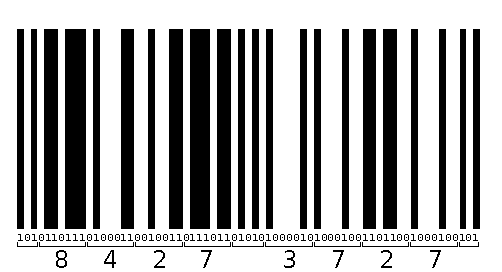
\includegraphics[width=\linewidth]{images/ean8_example_2}
    \captionof{figure}{EAN-8 example ("\texttt{84273727}")}
    \label{fig:ean8_ex}
  \end{minipage}
\end{minipage}

\subsubsection{EAN-13}
\label{sss:ean13}

EAN-13 follows the same principles as EAN-8. The structure of such a code is the following:

\def\arraystretch{1.5}
\begin{table}[H]
  \centering
  \begin{tabu}{|[2pt]c|c|c|c|c|c|c|c|c|c|c|c|c|c|c|[2pt]}
    \tabucline[2pt]{-}
    \multirow{2}{*}{left} & A & A & A & A & A & A & \multirow{2}{*}{mid} & \multirow{2}{*}{C} & \multirow{2}{*}{C} & \multirow{2}{*}{C} & \multirow{2}{*}{C} & \multirow{2}{*}{C} & \multirow{2}{*}{C} & \multirow{2}{*}{right}\\
    \cline{2-7}
    & B & B & B & B & B & B & & & & & & & & \\
    \tabucline[2pt]{-}
  \end{tabu}
  \caption{EAN-13 structure}
  \label{tab:ean13_struct}
\end{table}
\def\arraystretch{1}

This has only 12 places for elements, 6 A/B and 6 C. The 13th digit (in reality the first) is encoded in the pattern of A and B elements. Here is the list of patterns corresponding to each digit:

\def\arraystretch{1.5}
\begin{table}[H]
  \centering
  \begin{tabu}{|[2pt]c|c|[2pt]c|c|[2pt]}
    \tabucline[2pt]{-}
    Digit & Pattern & Digit & Pattern\\
    \tabucline[2pt]{-}
    0 & AAAAAA & 5 & ABBAAB \\
    \hline
    1 & AABABB & 6 & ABBBAA \\
    \hline
    2 & AABBAB & 7 & ABABAB \\
    \hline
    3 & AABBBA & 8 & ABABBA \\
    \hline
    4 & ABAABB & 9 & ABBABA \\
    \tabucline[2pt]{-}
  \end{tabu}
  \caption{EAN-13 1st digit patterns}
  \label{tab:ean13_patterns}
\end{table}
\def\arraystretch{1}

It can be noticed that the first element is always an A so that reading direction can easily be determined.

Let's illustrate EAN-13 by encoding the value "978294062105".


\begin{enumerate}
  \item Calculate the checksum digit:
  \def\arraystretch{1.5}
  \begin{table}[H]
    \centering
    \begin{tabu}{c|c|c|c|c|c|c|c|c|c|c|c|c|c}
      %\hline
        & 9 & 7 & 8 & 2 & 9 & 4 & 0 & 6 & 2 & 1 & 0 & 5 & \\
      %\hline
      x & 1 & 3 & 1 & 3 & 1 & 3 & 1 & 3 & 1 & 3 & 1 & 3 & \\
      \tabucline[2pt]{-}
      + & 9 &21 & 8 & 6 & 9 &12 & 0 &18 & 2 & 3 & 0 &15 & = 103 \\
      %\hline
    \end{tabu}
    \caption{Luhn Formula (EAN-13 example)}
    \label{tab:luhn_ean13_ex}
  \end{table}
  \def\arraystretch{1}

  Thus the last digit is $10 - (103 \textrm{ mod } 10) = 10 - 3 = 7$.

  \item Get the pattern corresponding to the first digit: 9 $\rightarrow$ ABBABA

  \item Take the corresponding element for each digit
  \def\arraystretch{1.5}
  \begin{table}[H]
    \centering
    \begin{tabu}{|[2pt]c|c|c|[2pt]|[2pt]c|c|c|[2pt]}
      \tabucline[2pt]{-}
      Char. & Type & Element & Char. & Type & Element \\
      \tabucline[2pt]{-}
      7 & A & 0111011 & 6 & C & 1010000\\
      \hline
      8 & B & 0001001 & 2 & C & 1101100\\
      \hline
      2 & B & 0011011 & 1 & C & 1100110\\
      \hline
      9 & A & 0001011 & 0 & C & 1110010\\
      \hline
      4 & B & 0011101 & 5 & C & 1001110\\
      \hline
      0 & A & 0001101 & 7 & C & 1000100\\
      \tabucline[2pt]{-}
    \end{tabu}
    \caption{EAN-13 example elements}
    \label{tab:ean13_elmt_ex}
  \end{table}
  \def\arraystretch{1}

  \item Add the delimiters "101" at each end and "01010" between both halves of the code.
  \item For each 1, draw a black bar and for each 0 a white one.

  \begin{figure}[H]
    \centering
    
\includegraphics[width=0.5\linewidth]{images/ean13_example}
    \caption{EAN-13 example ("\texttt{9782940621057}")}
    \label{fig:ean13_ex}
  \end{figure}
\end{enumerate}

  \section{Application in Python}
\label{sec:barcode_python}

In this section, we will implement barcode generation in Python. We will first program a "Code-39" encoder, then an EAN-8 and finally an EAN-13.

\subsection{Code-39}
\label{ssec:code39_py}

This type of code being just a matter of translating each character to a particular group of wide and narrow stripes, the implementation is quite simple.

We first create a dictionary holding the codes for each character.

\begin{minted}[frame=single]{python}
code39_dict = {
    "A": "100001001", "B": "001001001",
    "C": "101001000", "D": "000011001",
    "E": "100011000", "F": "001011000",
    "G": "000001101", "H": "100001100",
    "I": "001001100", "J": "000011100",
    "K": "100000011", "L": "001000011",
    "M": "101000010", "N": "000010011",
    "O": "100010010", "P": "001010010",
    "Q": "000000111", "R": "100000110",
    "S": "001000110", "T": "000010110",
    "U": "110000001", "V": "011000001",
    "W": "111000000", "X": "010010001",
    "Y": "110010000", "Z": "011010000",
    "0": "000110100", "1": "100100001",
    "2": "001100001", "3": "101100000",
    "4": "000110001", "5": "100110000",
    "6": "001110000", "7": "000100101",
    "8": "100100100", "9": "001100100",
    " ": "011000100", "-": "010000101",
    "$": "010101000", "%": "000101010",
    ".": "110000100", "/": "010100010",
    "+": "010001010", "*": "010010100"
}
\end{minted}

To convert a string, we map each character to its corresponding binary representation and join the resulting codes with "0" in between.

\begin{minted}[frame=single]{python}
def code39(text):
    text = text.upper()
    text = map(lambda c: code39_dict[c], text)
    return "0".join(text)
\end{minted}

We will also need a function to render the barcode. For this, we will use the Pygame module.

\begin{minted}[frame=single]{python}
def draw_barcode(barcode, win):
    barcode = list(map(int, barcode))
    width = win.get_width()*0.8
    height = win.get_height()*0.5
    thicks = sum(barcode)
    thins = len(barcode)-thicks
    bar_w = width/(thicks*2+thins)

    win.fill((255,255,255))
    x = win.get_width()*0.1
    y = win.get_height()*0.25

    for i, c in enumerate(barcode):
        w = 2*bar_w if c else bar_w
        if i%2 == 0:
            pygame.draw.rect(win, (0,0,0), [x, y, w, height])

        x += w
\end{minted}

The full python script can be found in appendix \ref{app:code39_py} or on \hreffn{https://github.com/LordBaryhobal/5D\_Heredero\_Louis\_TM2022/blob/main/python/code39.py}{GitHub}.

\subsection{EAN-8}
\label{ssec:ean8_py}

The first step to create an EAN-8 barcode is to compute the check digit with Luhn's formula.
To make this function also usable for EAN-13, we need to redefine the formula as such:

\begin{enumerate}
  \item Multiply each digit by the alternating factors 1 and 3 starting with 3 \textbf{from the end}.

  \item Add them together then take the modulo ten and subtract the result from 10.

  \item If the result is equal to 10, change it to 0.
\end{enumerate}

%Since this function will also be used for EAN-13, with only the factors changing, we will make it general enough.

In python, the function multiplies the i\textsuperscript{th} to last digit by: \[
  \text{factor} = 3 - (i\ mod\ 2) * 2
\]
which basicly is step 1 above.

\def\arraystretch{1.5}
\begin{table}[H]
  \centering
  \begin{tabu}{|[2pt]c|[2pt]c|c|c|c|c|c|[2pt]}
    \tabucline[2pt]{-}
    i & ... & 4 & 3 & 2 & 1 & 0 \\
    \hline
    factor & ... & 3 & 1 & 3 & 1 & 3 \\
    \tabucline[2pt]{-}
  \end{tabu}
  \caption{Python Luhn formula example}
  \label{tab:luhn_py_ex}
\end{table}
\def\arraystretch{1}

%\begin{minipage}{\linewidth}
\begin{minted}[frame=single]{python}
def luhn(digits):
    checksum = sum([
        digits[-i-1]*(3-i%2*2)
        for i in range(len(digits))
    ])
    ctrl_key = 10 - checksum%10
    if ctrl_key == 10:
        ctrl_key = 0

    return ctrl_key
\end{minted}
%\end{minipage}

Both code types also need the table of elements:

\begin{minted}[frame=single]{python}
A = [
    0b0001101,
    0b0011001,
    0b0010011,
    0b0111101,
    0b0100011,
    0b0110001,
    0b0101111,
    0b0111011,
    0b0110111,
    0b0001011
]

# XOR 0b1111111
C = list(map(lambda a: a^127, A))

# Reverse bit order
B = list(map(lambda c: int(f"{c:07b}"[::-1], 2), C))
\end{minted}

The following function converts a number to the list of its bits:
\begin{minted}[frame=single]{python}
def bin_list(n):
    return list(map(int, f"{n:07b}"))
\end{minted}

Finally, the encoding function:
\begin{minted}[frame=single]{python}
def ean8(digits):
    digits.append(luhn(digits))
    elmts = []

    elmts += [1,0,1] #delimiter
    for digit in digits[:4]:
        elmts += bin_list(A[digit])

    elmts += [0,1,0,1,0] #middle delimiter
    for digit in digits[4:]:
        elmts += bin_list(C[digit])

    elmts += [1,0,1] #delimiter
    return elmts
\end{minted}

We will use a similar function as in \autoref{ssec:code39_py} to render the barcode

\begin{minted}[frame=single]{python}
def draw_barcode(barcode, win):
    width = win.get_width()*0.8
    height = win.get_height()*0.5
    bar_w = width/len(barcode)

    win.fill((255,255,255))
    x = win.get_width()*0.1
    y = win.get_height()*0.25

    for c in barcode:
        if c:
            pygame.draw.rect(win, (0,0,0), [x, y, bar_w, height])

        x += bar_w
\end{minted}

The full python script can be found in appendix \ref{app:ean_py} or on \hreffn{https://github.com/LordBaryhobal/5D\_Heredero\_Louis\_TM2022/blob/main/python/ean.py}{GitHub}

\subsection{EAN-13}
\label{ssec:ean13_py}

The main difference with EAN-8 is the encoding of the first digit, using an A/B pattern. We will create a list of these patterns:

\begin{minted}[frame=single]{python}
ean13_patterns = [
    "AAAAAA",
    "AABABB",
    "AABBAB",
    "AABBBA",
    "ABAABB",
    "ABBAAB",
    "ABBBAA",
    "ABABAB",
    "ABABBA",
    "ABBABA"
]
\end{minted}

And the appropriate encoding function:

\begin{minted}[frame=single]{python}
def ean13(digits):
    pattern = ean13_patterns[digits[0]]
    digits.append(luhn(digits))
    elmts = []

    elmts += [1,0,1] #delimiter
    for d in range(1,7):
        _ = A if pattern[d-1] == "A" else B
        digit = digits[d]
        elmts += bin_list(_[digit])

    elmts += [0,1,0,1,0] #middle delimiter
    for digit in digits[7:]:
        elmts += bin_list(C[digit])

    elmts += [1,0,1] #delimiter
    return elmts
\end{minted}

The full python script can be found in appendix \ref{app:ean_py} or on \hreffn{https://github.com/LordBaryhobal/5D\_Heredero\_Louis\_TM2022/blob/main/python/ean.py}{GitHub}


  \chapter{QR-Codes}
\label{chap:qr_origin}

\section{Origin}
\label{sec:qr_origin}

Eventhough barcodes have conquered the world, they still have some major issues.
First of all, their capacity is rather limited, allowing only a maximum of about twenty characters to be encoded in a practical format.
Secondly, they can only store a small group of characters, some even only numbers.
And finally, they require the reading device to be in a roughly parallel orientation with respect to the code in order to read it.

For these reasons, the Japanese company named DENSO WAVE started developing a new type of 2D code.
Indeed, a barcode is one-dimensional - that is, the information is encoded on a single axis.
What DENSO WAVE tried was a two-dimensional matrix of data.

The result of their research and development became the well-known "QR-Code", which stands for Quick-Response code. They were first used in Toyota factories to track car parts\cite{qrcode_history}.
With the desire to offer this technology to the largest number of people, the company decided not to keep it private but rather make it open-source.
It later became a norm in many countries and is now specified by the ISO/IEC~18004 standard \cite{ISO18004}.

QR-Codes address all the above-mentioned problems related to barcodes.

\subsection*{Data type}

They allow the encoding of either numbers, text, raw binary data and even Kanji characters\footnote{Kanji are the characters used to write Japanese}. Therefore they can be used in a great variety of contexts, for example to identify objects, to conviniently share a URL or even a small image.

\subsection*{Information density}

They allow dense information storage.

\def\arraystretch{1.5}
\begin{table}[H]
  \centering
  \begin{tabu}{|[2pt]c|c|[2pt]}
    \tabucline[2pt]{-}
    Type & Number of "characters" \\
    \tabucline[2pt]{-}
    Numerical & 7'089 \\
    \hline
    Alphanumerical & 4'296 \\
    \hline
    Bytes & 2'953 \\
    \hline
    Kanji & 1'817 \\
    \tabucline[2pt]{-}
  \end{tabu}
  \caption{Maximum amount of data in a QR-Code \cite{ISO18004}}
  \label{tab:qr_max_data}
\end{table}
\def\arraystretch{1}

The alphanumerical type can only encode the following characters:
\begin{center}
  \texttt{0123456789ABCDEFGHIJKLMNOPQRSTUVWXYZ \$\%*+-./:}
\end{center}

\subsection*{Reading freedom}

Thanks to finder patterns, they can be read in any orientation, even with perspective. Taking into account the great progress which happened during the last 30 years in the field of cameras and mobile phones, QR-Codes can now be scanned in a matter of milliseconds, no matter the angle of the camera.

\subsection*{Error detection and correction}

The other main advantage of QR-Codes is the embedded error detection and correction system.

They come in four different levels of error correction:
\begin{itemize}
  \item L (low): 7\%
  \item M (medium): 15\%
  \item Q (quartile): 25\%
  \item H (high): 30\%
\end{itemize}

A higher level indicates a greater amount of redundancy and an ability to recover a greater part of a damaged code. This principle is often used to add a custom icon at the center of the QR-Code, since the reader will still be able to scan it and reconstruct the hidden part.

  \section{How it works}
\label{sec:qr_functioning}

Graphically, QR-Codes are composed of black and white squares called "modules". Each module represents a binary bit, black meaning 1, white meaning 0.

Similarly to \autoref{sec:barcode_functioning}, we will only describe the encoding phase.

To make the following explanations easier to follow, we will use a concrete value.

Let's encode the string "Hello, World!" with level "M" of error correction.

\subsection{Data type}
\label{ssec:qr_data_type}

The first step is to choose the appropriate data type for encoding. In our case, we can't use the numerical format since there are letters, nor can we use the alphanumerical, because of the exclamation mark and lowercase letters. Thus, the most suitable encoding is the byte format.

Note that these different formats exist to optimize encoding to take the least possible space, so it is recommended to choose the minimum required format to avoid unecessarily big QR-Codes.

The first 4 bits of data in our code will be the format used. Numerical is 1, alphanumerical is 2, byte is 4 and kanji is 8. In our case, the format indicator will be "0100".

\subsection{Version}
\label{ssec:qr_version}

QR-Codes come in a number of sizes, called "versions". Version 1 (the smallest) is a 21x21 grid, version 2 a 25x25, version 3 29x29, and so on, up to version 40 (the largest) which is a 157x157 matrix.

To know which size our code will be, we have to refer to table \ref{tab:qr_versions} indicating which version is needed for a certain amount of data.

Our string contains 13 characters, that is 13 bytes (in ISO-8859-1) and will be encoded using the byte format with level "M" of error correction. Thus the final code will be of version 1.

\subsection{Character count indicator}
\label{ssec:qr_char_count_ind}

Before encoding our data, we need to create a header stating the total character count. For that, the length is converted to its binary representation of $n$ bits, where $n$ depends on the version and encoding mode, as shown in table \ref{tab:qr_char_count_len}.

\def\arraystretch{1.5}
\begin{table}[H]
  \centering
  \begin{tabu}{|[1pt]c|c:c:c:c|[1pt]}
    \tabucline[1pt]{-}
    Version & Num. & Alpha. & Byte & Kanji\\
    \tabucline[1pt]{-}
    1 to 9 & 10 & 9 & 8 & 8 \\
    \hline
    10 to 26 & 12 & 11 & 16 & 10 \\
    \hline
    27 to 40 & 14 & 13 & 16 & 12 \\
    \tabucline[1pt]{-}
  \end{tabu}
  \caption{Bit length of character count indicator}
  \label{tab:qr_char_count_len}
\end{table}
\def\arraystretch{1}

In our example, the number of characters is 13, which means the character count indicator is "00001101".

\subsection{Data encoding}
\label{ssec:qr_encoding}

The following step is to convert the data to binary. The method used differs for each format.

\subsubsection{Numerical}
\label{sssec:qr_encoding_num}

\begin{enumerate}
  \item Split the number into 3-digit groups
  \item For each group, convert the number to binary, padded to:
  \begin{itemize}
    \item 10 bits if there are 3 digits (most groups)
    \item 7 bits if there are 2 digits (only sometimes for the last group)
    \item 4 bits if there is only one digit (only sometimes for the last group)
  \end{itemize}
  \item Join the resulting bits end to end
\end{enumerate}

\subsubsection{Alphanumerical}
\label{sssec:qr_encoding_alpha}

\begin{enumerate}
  \item Split the string into 2-character groups
  \item For each group:
  \begin{enumerate}
    \item Take the first character's index in list \ref{tab:qr_alphanum} and multiply it by 45
    \item Take the second character's index in list \ref{tab:qr_alphanum}
    \item Add them together and convert the result to an 11-bit number
  \end{enumerate}
  \item If the string has an odd number of characters, take the index of the last character and convert it to a 6-bit number
\end{enumerate}

\subsubsection{Byte}
\label{sssec:qr_encoding_byte}

\begin{enumerate}
  \item Encode the data in ISO-8859-1 (latin-1)
  \item Join the 8-bit binary representation of each character end to end
\end{enumerate}

\subsubsection{Kanji}
\label{sssec:qr_encoding_kanji}

\begin{enumerate}
  \item Encode the data in JIS X 0208 (each character is encoded on 2 bytes)
  \item For each character (= pair of bytes):
  \begin{enumerate}
    \item If the value is between 0x8140 and 0x9FFC, subtract 0x8140 \\
    Otherwise, if the value is between 0xE040 and 0xEBBF, subtract 0xC140
    \item Multiply the most significant byte by 0xC0
    \item Add the most significant byte to the least significant
    \item Join the 13-bit binary representation of each sum end to end
  \end{enumerate}
\end{enumerate}

\subsubsection{Example}
\label{sssec:qr_encoding_ex}

For our example, following the byte encoding format, we get:

\def\arraystretch{1.2}
\begin{center}
  \begin{tabu}{|c|c|c|c|c|}
    \hline
    \textbf{01000000} & \textbf{1101}0100 & 10000110 & 01010110 & 11000110 \\
    \hline
    11000110 & 11110010 & 11000010 & 00000101 & 01110110 \\
    \hline
    11110111 & 00100110 & 11000110 & 01000010 & 0001 \\
    \hline
  \end{tabu}
\end{center}
\def\arraystretch{1}

Note that the format and character count indicator have been added at the begginning (bolded bits).

The resulting binary string needs to be padded before continuing to the next step. This is done in a fourfold process:
\begin{enumerate}
  \item Get the total number of bits in the final code by multiplying column "Data codewords" of table \ref{tab:qr_error_correction} by eight\footnote{A codeword is equivalent to an 8-bit byte}. Let that be $B$ and let $b$ be the number of data bits we already have
  \item Add $B-b$ 0s, but at most 4
  \item Add 0s so that $b$ is a multiple of 8, if not already
  \item If $b < B$, fill the remaining bits with the alternating bytes "\texttt{11101100}" and "\texttt{00010001}"
\end{enumerate}

In our example, we already have 116 data bits on 128 as per table \ref{tab:qr_error_correction} (version 1, level M). Thus we add four 0s, increasing $b$ to 120. We don't need to add other 0s since it is already a multiple of 8. Finally we fill the remaining 8 bits with the alternating padding bytes. The result is:

\def\arraystretch{1.2}
\begin{center}
  \begin{tabu}{|c|c|c|c|c|}
    \hline
    01000000 & 11010100 & 10000110 & 01010110 & 11000110 \\
    \hline
    11000110 & 11110010 & 11000010 & 00000101 & 01110110 \\
    \hline
    11110111 & 00100110 & 11000110 & 01000010 & 00010000 \\
    \hline
    11101100 & & & & \\
    \hline
  \end{tabu}
\end{center}
\def\arraystretch{1}

\subsection{Error correction}
\label{ssec:qr_error_corection}

Now that we have encoded our data, we need to create additional error correction codewords. QR-Codes use what is called the Reed-Solomon algorithm to detect and correct potential errors in a scanned code. This algorithm is explained in more details in \autoref{sec:reed_solomon}.

According to table \ref{tab:qr_error_correction}, we need a certain number of error correction codewords (column "Error correction codewords per block"). Let this number be n.

For that, we create a generator polynomial: \[
  \prod_{i = 0}^{n-1} (x + 2^i)
\]
Note that the calculation are done in a Galois field, as explained in \autoref{sec:reed_solomon}.

Encoded data now needs to be split in B1 blocks (see table \ref{tab:qr_error_correction}, column "Blocks in group 1"). Each block contains C1 data codewords (see table \ref{tab:qr_error_correction}, column "Data codewords per group 1 blocks").

For each block:
\begin{enumerate}
  \item Convert each codeword to its decimal value (in the Galois field) and let that be the coefficients of a "message" polynomial.
  \item Divide this polynomial by the generator polynomial created earlier.
  \item Convert the coefficients of the remainder to their 8-bit binary representation and let these be the error correction codewords for this block.
\end{enumerate}

If group 2 has a non-null amount of data codewords, do the same steps for column "Blocks in group 2" (B2) and "Data codewords per group 2 blocks" (C2).

For our example, n = 10, B1 = 1, C1 = 16, B2 = 0, C2 = 0.
The generator polynomial has the coefficients: \[
  1, 216, 194, 159, 111, 199, 94, 95, 113, 157, 193
\]

We only have one block with 16 codewords, so our "message" polynomial will have the coefficients: \[
  64, 212, 134, 86, 198, 198, 242, 194, 5, 118, 247, 38, 198, 66, 16, 236
\]

Dividing it by the generator polynomial, we get a remainder with the coefficients: \[
  215, 92, 247, 55, 155, 152, 59, 246, 87, 124
\]

that we convert to binary bytes, giving us:
\def\arraystretch{1.2}
\begin{center}
  \begin{tabu}{|c|c|c|c|c|}
    \hline
    11010111 & 01011100 & 11110111 & 00110111 & 10011011 \\
    \hline
    10011000 & 00111011 & 11110110 & 01010111 & 01111100 \\
    \hline
  \end{tabu}
\end{center}
\def\arraystretch{1}

\subsection{Interleaving}
\label{ssec:qr_interleaving}

Now that we have computed the error correction codewords, we need to arrange them in a certain manner with the data codewords. The codewords go in the following order:

%TODO: improve this table
\def\arraystretch{1.2}
\begin{center}
  \begin{tabu}{|[2pt]c|c|c|c|c||c|c|c|c|[2pt]}
    \tabucline[2pt]{-}
    Data & \rot{Codeword 1} & \rot{Codeword 2} & \rot{Codeword 3} & \rot{Codeword 4} & \shortstack[c]{Error \\ correction} & \rot{Codeword 1} & \rot{Codeword 2} & \rot{Codeword 3}\\
    \hline
    Block 1 & 1 & 5 &  9 &  x & Block 1 & 15 & 19 & 23 \\
    \hline
    Block 2 & 2 & 6 & 10 &  x & Block 2 & 16 & 20 & 24 \\
    \hline
    Block 3 & 3 & 7 & 11 & 13 & Block 3 & 17 & 21 & 25 \\
    \hline
    Block 4 & 4 & 8 & 12 & 14 & Block 4 & 18 & 22 & 26 \\
    %\hline
    %... & ... & ... & ... & ... & ... & ... & ... & ... \\
    \tabucline[2pt]{-}
  \end{tabu}
\end{center}
\def\arraystretch{1}

In this example, B1 = 2, C1 = 3, B2 = 2, C2 = 4.

In our case, since we only have 1 data block, the error correction codewords are simply appended after the data codewords.

Similarly to step \ref{ssec:qr_encoding} (\nameref{ssec:qr_encoding}), we need to pad the end result with a certain number of 0s before continuing. This number is given by the following table:

\def\arraystretch{1.2}
\begin{center}
  \begin{tabu}{|[2pt]c|c|[2pt]}
    \tabucline[2pt]{-}
    Version & Number of 0s to add\\
    \hline
    2 to 6 & 7 \\
    \hline
    14 to 20 & 3 \\
    \hline
    21 to 27 & 4 \\
    \hline
    28 to 34 & 3 \\
    \tabucline[2pt]{-}
  \end{tabu}
\end{center}
\def\arraystretch{1}

Our example code is a version 1 so we don't need to add any 0.

\subsection{Separators and finder patterns}
\label{ssec:qr_sep_finder}

Data has been encoded and now starts the placement phase, that is the creation of the black and white matrix.

First of all, the matrix' size (in number of modules) is given by the following formula: \[
  (V-1)*4 + 21
\]
where $V$ is the version.

The ISO standard\cite{ISO18004} also states that a 4-module wide margin (silence zone) must be respected all around the code. This allows scanners to easily identify and locate a QR-Code in an image.

The distinctive elements of QR-Codes are of course their three large corner squares. These are called "finder patterns" and are used by the reading device to find the code and correct the perspective. They also provide information on the rotation of the image and the width of individual modules. Finder patterns are 7x7 black squares, containing a 5x5 white square, encircling itself a 3x3 black square. They are put in the top-left, top-right and bottom-left corners of the matrix.

Additionally, they are separated from the rest of the code by a 1-module thick white line called a separator.

For our version 1 QR-Code, this steps yields the following 21x21 matrix:

\begin{figure}[H]
  \centering
  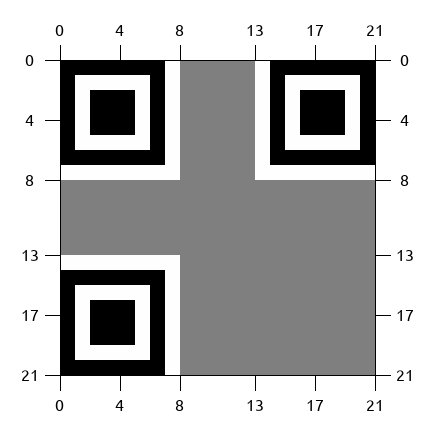
\includegraphics[width=0.4\textwidth]{images/qr_sep_finder}
  \caption{QR-Code example: separators and finder patterns}
  \label{fig:qr_sep_finder}
\end{figure}

\subsection{Alignment patterns}
\label{ssec:qr_alignment}

The next element to add are the alignment patterns. These are similar to finder patterns but are only 5x5. They are spread across the whole code and provide reference points for the scannnig device to improve reliability. The larger the code, the more alignment patterns are needed. Their positions depend on the version and are referenced in table \ref{tab:qr_alignment}. This table lists all possible x and y coordinates for the patterns. This means that for version 2, the alignment patterns are located at (6,6), (6,18), (18,6) and (18,18). A pattern will only be present if the area it covers is still empty (i.e. it doesn't overlap with the separators and finder patterns).

Since our example is a version 1 QR-Code, no alignment pattern is needed (see figure \ref{fig:qr_reserved} for version 10 code with alignment patterns).

\subsection{Timing pattern}
\label{ssec:qr_timing}

An additional element helping the scanner and improving readability is the timing pattern. It consists of a alternating black and white stripe joining the bottom-left and top-left finder pattern, and the top-left and top-right.

The pattern is aligned to the right and bottom borders of the top-left finder patterns, starting with white on the separators.

\begin{figure}[H]
  \centering
  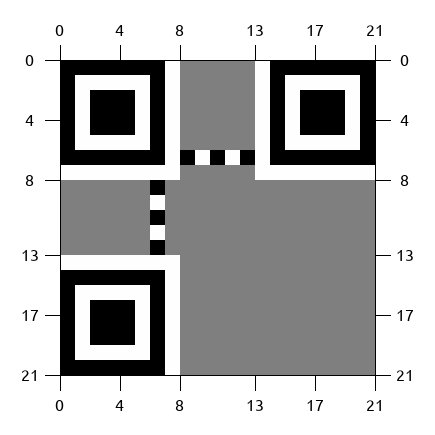
\includegraphics[width=0.4\textwidth]{images/qr_timing}
  \caption{QR-Code example: timing patterns}
  \label{fig:qr_timing}
\end{figure}

\subsection{Reserved area}
\label{ssec:qr_reserved}

Some areas of the matrix are also reserved for format information which will be added later. This corresponds to the modules around the top-left finder pattern, the modules on the right of the bottom-left pattern and those just below the top-right one.

Additionally, for versions greater than 6, a 3x6 zone on the left of the top-right finder pattern plus a 6x3 above the bottom-left one are reserved for version information.

Figure \ref{fig:qr_reserved} shows an example of these reserved areas (in light gray) for a version 10 QR-Code (left) and for our example (right).

\begin{figure}[H]
  \centering
  \raisebox{-0.5\height}{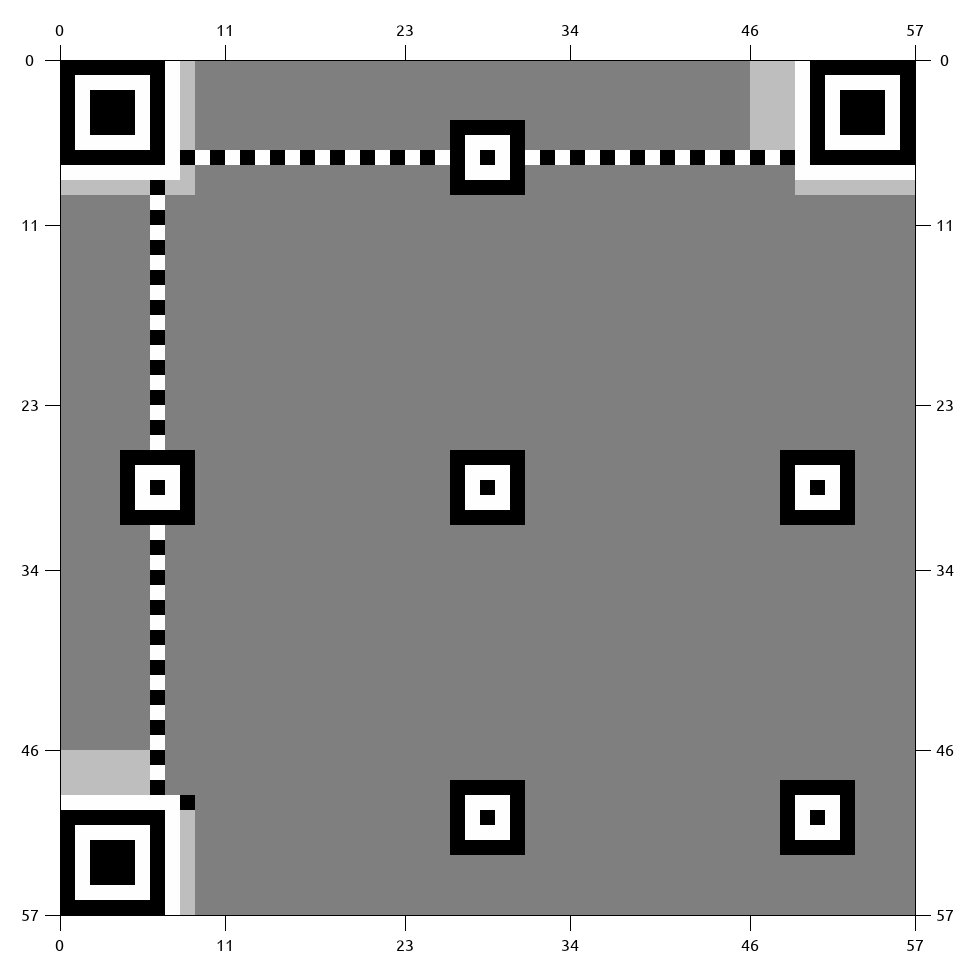
\includegraphics[width=0.5\textwidth]{images/qr_reserved_example}}
  \raisebox{-0.5\height}{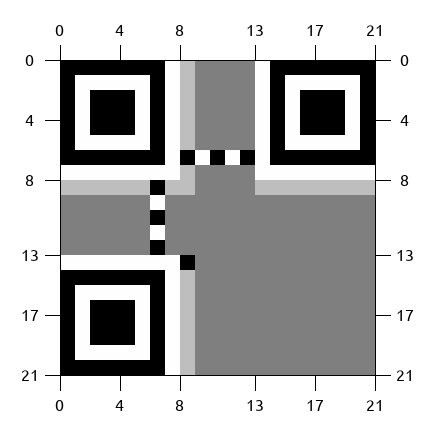
\includegraphics[width=0.4\textwidth]{images/qr_reserved}}
  \caption{QR-Code example: reserved areas}
  \label{fig:qr_reserved}
\end{figure}

A black module is also set next to the bottom-left finder pattern, on the right of its top-right corner. Its coordinates are the following:
\begin{math}
  \begin{cases}
    x = 8 \\
    y = 4V + 9
  \end{cases}
\end{math}
where $V$ is the version.

\subsection{Data placement}
\label{ssec:qr_placement}

The matrix is now ready to receive the data bit string. The placement is done in zigzags, starting from the bottom-right, going up. Each byte is placed in a 2 modules wide region in a staggered manner. When a pattern, separator or reserved area is encountered, the position is skipped and the process continues further.

Figures \ref{fig:qr_plcmt_byte_up} and \ref{fig:qr_plcmt_byte_down} represent the way a byte is layed out when going up or down.

Figures \ref{fig:qr_plcmt_reserved} and \ref{fig:qr_plcmt_turning} show how skipping and turning are processed.

When encountering the vertical timing pattern, that column is entirely skipped and the placement continues on the next one. For each byte, the bits are layed from Most Significant bit (MSB) to Least Significant Bit (LSB).

\begin{figure}[H]
  \centering
  \begin{subfigure}{0.3\textwidth}
    \centering
    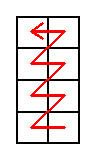
\includegraphics[width=0.5\textwidth]{images/qr_plcmt_byte_up}
    \caption{Going up}
    \label{fig:qr_plcmt_byte_up}
  \end{subfigure}
  \begin{subfigure}{0.3\textwidth}
    \centering
    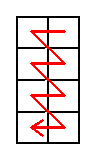
\includegraphics[width=0.5\textwidth]{images/qr_plcmt_byte_down}
    \caption{Going down}
    \label{fig:qr_plcmt_byte_down}
  \end{subfigure}
  \begin{subfigure}{0.3\textwidth}
    \centering
    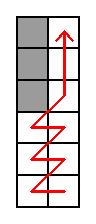
\includegraphics[width=0.5\textwidth]{images/qr_plcmt_reserved}
    \caption{Skipping reserved areas}
    \label{fig:qr_plcmt_reserved}
  \end{subfigure}
  \begin{subfigure}{0.3\textwidth}
    \centering
    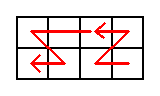
\includegraphics[width=0.7\textwidth]{images/qr_plcmt_turning}
    \caption{Turning at border}
    \label{fig:qr_plcmt_turning}
  \end{subfigure}
  \caption{QR-Code byte placement}
  \label{fig:qr_plcmt_byte}
\end{figure}

\begin{comment}
\begin{figure}[H]
  \centering
  \begin{subfigure}{0.3\textwidth}
    \centering
    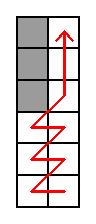
\includegraphics[width=0.3\textwidth]{images/qr_plcmt_reserved}
    \caption{Skipping reserved areas}
    \label{fig:qr_plcmt_reserved}
  \end{subfigure}
  \begin{subfigure}{0.6\textwidth}
    \centering
    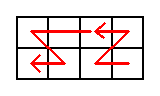
\includegraphics[width=0.5\textwidth]{images/qr_plcmt_turning}
    \caption{Turning at border}
    \label{fig:qr_plcmt_turning}
  \end{subfigure}
  \caption{QR-Code byte placement}
  \label{fig:qr_plcmt_byte_special}
\end{figure}
\end{comment}

If the available space if not fully filled after placing the data, the rest is filled with 0s\footnote{it shall be recalled that 0 means white and 1 means black}.

Our example QR-Code, once filled with data, looks like this:

\begin{figure}[H]
  \centering
  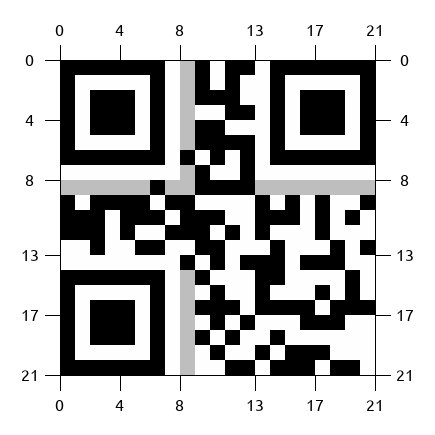
\includegraphics[width=0.4\textwidth]{images/qr_plcmt}
  \caption{QR-Code example: data placement}
  \label{fig:qr_plcmt}
\end{figure}

\subsection{Masking}
\label{ssec:qr_masking}

For optimal readability, it is important that certain patterns of modules don't appear inside the code. For example, there shouldn't be any shape resembling the finder or alignment patterns (i.e. modules with the ratio 1:1:3:1:1). Furthermore, a balanced amount of black compared to white is preferred for better decoding.

For this purpose, we need to apply a mask on the code, switching white for black modules and vice versa where it applies. QR-Codes have 8 different masks which can be used. Obviously, these are only applicable on the data area and should not modify the timing, finder and alignment patterns.

To choose one, we will apply them one after the other on our current QR-Code, and evaluate the resulting code, giving it a penalty score for each undesired feature. Then, the mask with the lowest score will be chosen.

Figure \ref{fig:qr_masks} lists the different possible masks.
A black mask module means that the corresponding data module needs to be inverted.
The operator "//" is integer division.

\begin{figure}[H]
  \centering
  \begin{subfigure}{0.4\textwidth}
    \centering
    
\includegraphics[width=0.4\textwidth]{images/qr_mask_0}
    \caption{(x+y) mod 2 = 0}
    \label{fig:qr_mask_0}
  \end{subfigure}
  \begin{subfigure}{0.4\textwidth}
    \centering
    
\includegraphics[width=0.4\textwidth]{images/qr_mask_1}
    \caption{y mod 2 = 0}
    \label{fig:qr_mask_1}
  \end{subfigure}
  \begin{subfigure}{0.4\textwidth}
    \centering
    
\includegraphics[width=0.4\textwidth]{images/qr_mask_2}
    \caption{(x) mod 3 = 0}
    \label{fig:qr_mask_2}
  \end{subfigure}
  \begin{subfigure}{0.4\textwidth}
    \centering
    
\includegraphics[width=0.4\textwidth]{images/qr_mask_3}
    \caption{(x+y) mod 3 = 0}
    \label{fig:qr_mask_3}
  \end{subfigure}
  \begin{subfigure}{0.4\textwidth}
    \centering
    
\includegraphics[width=0.4\textwidth]{images/qr_mask_4}
    \caption{(y//2+x//3) mod 2 = 0}
    \label{fig:qr_mask_4}
  \end{subfigure}
  \begin{subfigure}{0.4\textwidth}
    \centering
    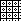
\includegraphics[width=0.4\textwidth]{images/qr_mask_5}
    \caption{((x*y) mod 2 + (x*y) mod 3) = 0}
    \label{fig:qr_mask_5}
  \end{subfigure}
  \begin{subfigure}{0.4\textwidth}
    \centering
    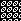
\includegraphics[width=0.4\textwidth]{images/qr_mask_6}
    \caption{((x*y) mod 2 + (x*y) mod 3) mod 2 = 0}
    \label{fig:qr_mask_6}
  \end{subfigure}
  \begin{subfigure}{0.4\textwidth}
    \centering
    
\includegraphics[width=0.4\textwidth]{images/qr_mask_7}
    \caption{((x+y) mod 2 + (x*y) mod 3) mod 2 = 0}
    \label{fig:qr_mask_7}
  \end{subfigure}
  \caption{QR-Code masks}
  \label{fig:qr_masks}
\end{figure}


\subsubsection{Evaluation}
\label{sssec:qr_mask_eval}

Evaluation of a mask is done thanks to 4 criteria.

They evaluate whether the code is easy to read or not. For example, criterion 3 gives a high penalty for every pattern with the same proportions as finder patterns to avoid confusion for the reading device.

Before applying a mask for evaluation, format and version information have do be added on the code, as described in sections \ref{ssec:qr_fmt_info} and \ref{ssec:qr_ver_info}.

\begin{enumerate}
  \item 5+ consecutive modules of the same color:

  If a line or column of 5 or more modules of the same color is found in the code, a penalty score is added. For a strip of $5 + i$ same colored modules, the penalty is worth $3 + i$ points.

  \item 2x2 blocks:

  Each 2x2 block of similar modules adds 3 points to the penalty score. Overlapping blocks are taken into account.

  \item 1:1:3:1:1:4 patterns:

  For each pattern with the ratios 1:1:3:1:1:4 or 4:1:1:3:1:1, a penalty of 40 points is given. This criterion takes into account the 4-module wide margins all around the code\footnote{see \autoref{ssec:qr_sep_finder}}. This means there are at least 18 correspondances in every code.

  \item Proportion of black and white modules:

  A penalty is attributed according to the deviation from a 50/50 distribution in black and white modules across the whole QR-Code. The calculation method is the following:
  \[ P = \lfloor 100 * B / (W*H) \rfloor \]
  \[ P_1 = P - P \textrm{ mod } 5 \]
  \[ P_2 = P_1 + 5 \]
  \[ S = \textrm{min}\left(\frac{|P_1 - 50|}{5}, \frac{|P_2 - 50|}{5}\right) * 10 \]
\end{enumerate}

where $B$ is the total number of black modules, $W$ and $H$ are the width and height of the QR-Code, and $S$ is the penalty score given for this criterion.

Applying this to our QR-Code, we can determine that the best mask is mask \ref{fig:qr_mask_5} with a score of 442. Figures \ref{fig:qr_mask_ex_eval_1} to \ref{fig:qr_mask_ex_eval_4} detail the penalties for each criterion.

\begin{figure}[H]
  \centering
  \begin{subfigure}{0.45\textwidth}
    \centering
    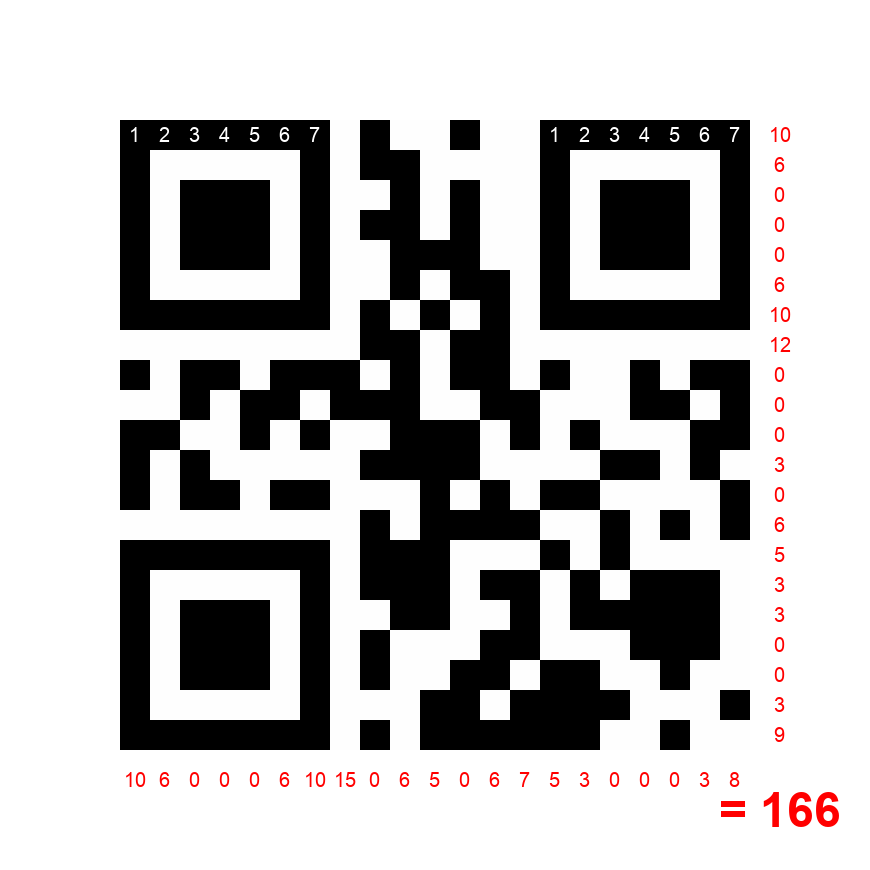
\includegraphics[width=\textwidth]{images/qr_mask_ex_eval_1}
    \caption{QR-Code example: mask evaluation (1)}
    \label{fig:qr_mask_ex_eval_1}
  \end{subfigure}
  \begin{subfigure}{0.45\textwidth}
    \centering
    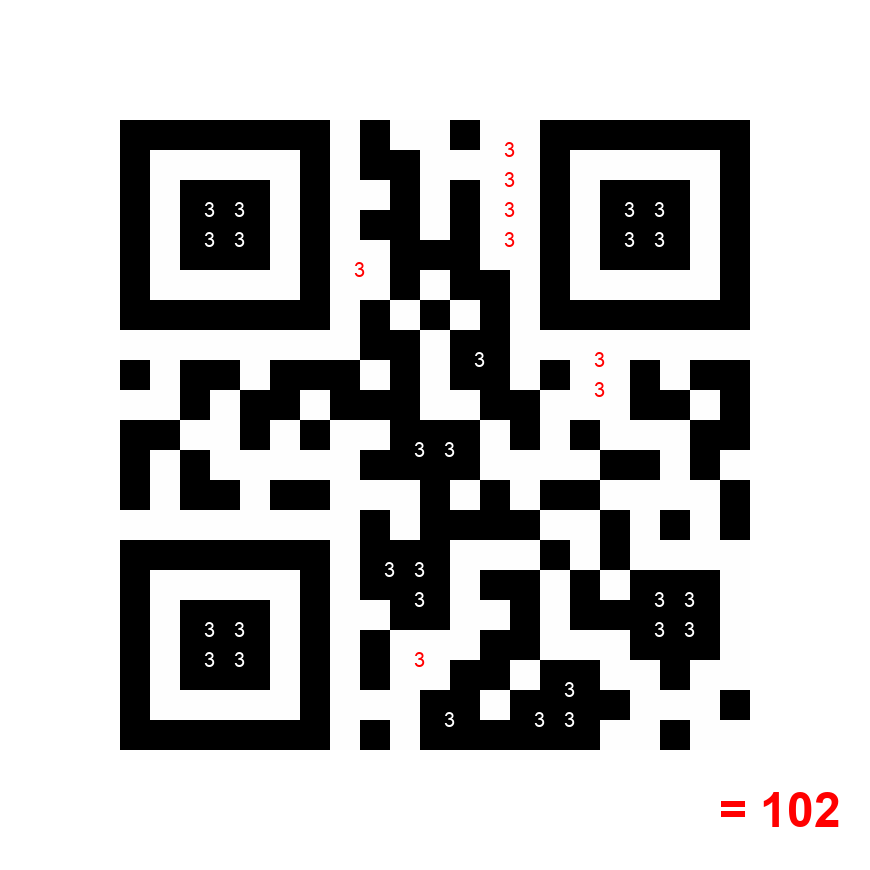
\includegraphics[width=\textwidth]{images/qr_mask_ex_eval_2}
    \caption{QR-Code example: mask evaluation (2)}
    \label{fig:qr_mask_ex_eval_2}
  \end{subfigure}
  \begin{subfigure}{0.45\textwidth}
    \centering
    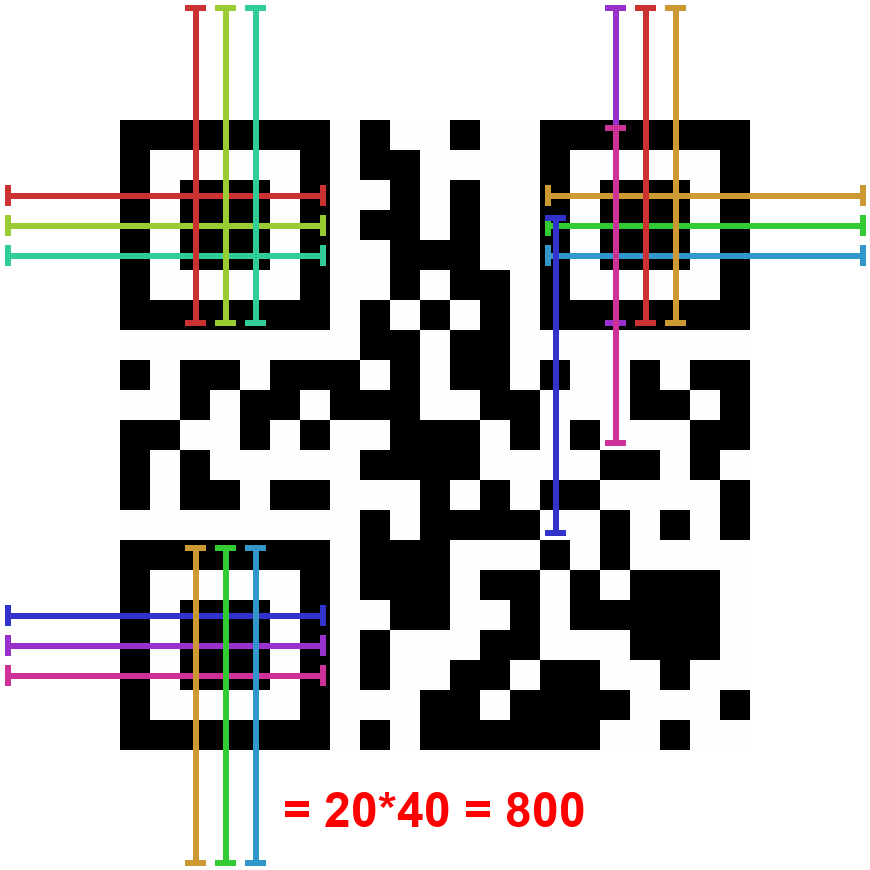
\includegraphics[width=\textwidth]{images/qr_mask_ex_eval_3}
    \caption{QR-Code example: mask evaluation (3)}
    \label{fig:qr_mask_ex_eval_3}
  \end{subfigure}
  \begin{subfigure}{0.45\textwidth}
    \centering
    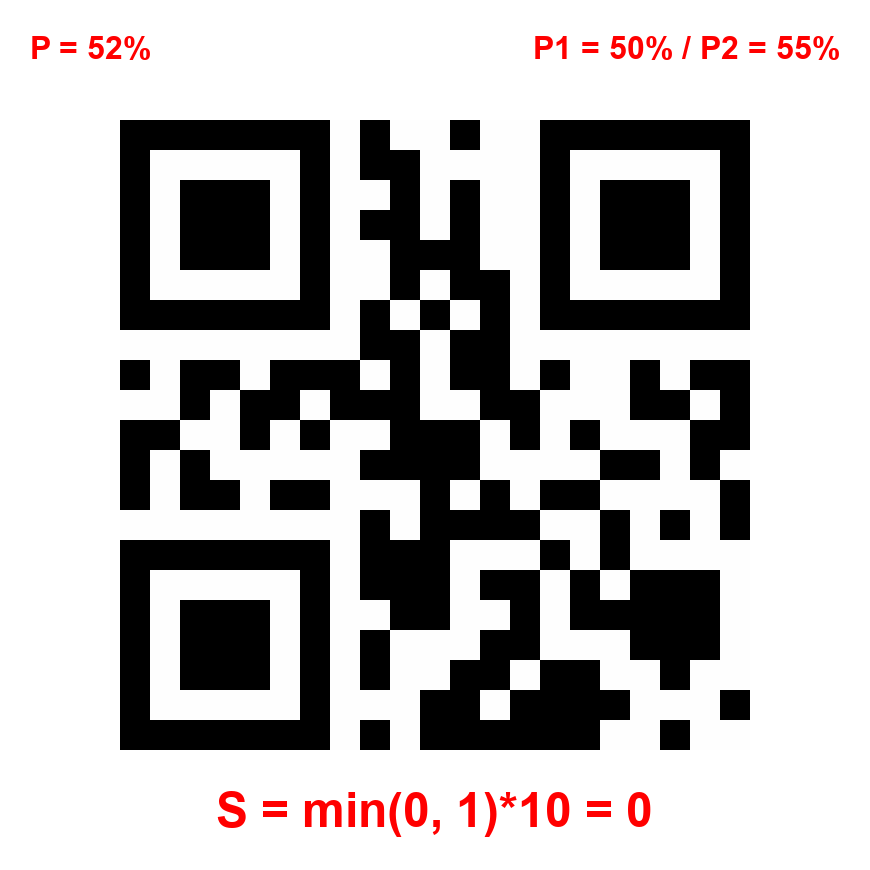
\includegraphics[width=\textwidth]{images/qr_mask_ex_eval_4}
    \caption{QR-Code example: mask evaluation (4)}
    \label{fig:qr_mask_ex_eval_4}
  \end{subfigure}
  \caption{QR-Code example: mask evaluation}
  \label{fig:qr_mask_ex_eval}
\end{figure}

\subsection{Format information}
\label{ssec:qr_fmt_info}

The last step to complete a fully functional QR-Code is to add the format information, and version information for versions bigger than 6.

First we need to create a format string containing the level of error correction and the mask used. The correction level is encoded on 2 bits as follows:

\begin{table}[H]
  \centering
  \begin{tabu}{|c|c|}
    \hline
    Level & Value (bin) \\
    \hline
    L & 01 \\
    \hline
    M & 00 \\
    \hline
    Q & 11 \\
    \hline
    H & 10 \\
    \hline
  \end{tabu}
  \caption{QR-Code error correction level indicator}
  \label{tab:qr_ec_ind}
\end{table}

Then the mask id is converted to a 3-bit binary number and appended to the error correction level indicator.

The string is padded by an additional 10 0s to make it 15 bits long.

Similarly to what has been done with data previously, the format string is complemented with error correction bits, this time using Bose-Chaudhuri-Hocquenghem (BCH) codes.
The principle is similar to the Reed-Solomon algorithm in that a message polynomial is divided by a generator polynomial. To create the message polynomial, each bit of the format string represents the coefficient of a term. The same applies for the generator polynomial, which is always derived from the binary number \texttt{10100110111}.
The generator polynomial is thus \[
  x^{10} + x^8 + x^5 + x^4 + x^2 + x + 1
\]

The division's remainder is then padded on the left with 0s to make it 10 bits long.

The final bit string is constructed by concatenating the format string with the error correction bits, and XORing\footnote{With the binary XOR operator} the result with the mask string \texttt{101010000010010}. This mask ensures the final format string is not made of only 0s.

Once calculated, the bit string is layed out in the reserved strips around the finder patterns, as shown in figure \ref{fig:qr_fmt_layout} (0 being the LSB and 14 the MSB)

\begin{figure}[H]
  \centering
  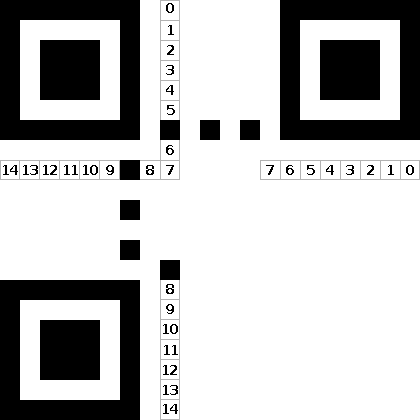
\includegraphics[width=0.4\textwidth]{images/qr_fmt_layout}
  \caption{QR-Code format information string layout}
  \label{fig:qr_fmt_layout}
\end{figure}

It is to be noted that format information appears twice, since its decoding is essential for reading the whole code.

In our case, the error correction indicator for level M is 00 and we used the mask with id 2, so our format string is \texttt{000100000000000}. Dividing it by the generator polynomial yields the remainder \texttt{1001101110}.

Adding it to the format string and XORing it with the mask string, we get \texttt{101111001111100}.

These bits are then put in the reserved areas of the matrix, making figure \ref{fig:qr_fmt_info}

\begin{figure}[H]
  \centering
  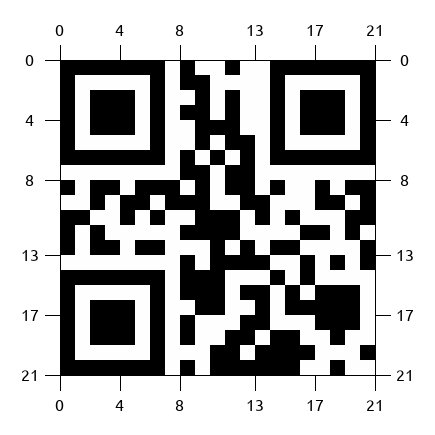
\includegraphics[width=0.4\textwidth]{images/qr_fmt_info}
  \caption{QR-Code example: format information}
  \label{fig:qr_fmt_info}
\end{figure}

Our QR-Code is now fully finished and can be scanned.

\subsection{Version information}
\label{ssec:qr_ver_info}

For QR-Codes of version 7 and bigger, additional data is added to state the code's version.

To generate the version string, first convert the version to its 6 bit binary representation. Then append the remainder of the division by the generator polynomial \[
  x^{12} + x^{11} + x^{10} + x^9 + x^8 + x^5 + x^2 + 1
\] padded on the left to 12 bits, following the same methods as for format information.

This string is then put in the two reserved 6x3 and 3x6 rectangles. The LSB is placed in the top-left corner of the rectangles. For the top-right area, the string goes down, then to the right. For the bottom-left rectangle, the string goes to the right, then down.

  \section{Application in Python}
\label{sec:qr_python}

In this section, we will look at my Python QR-Code generator implementation.
For the sake of brevity, only some specific parts of the program will be commented.

\subsection{Python features}
\label{ssec:qr_py_features}

The script takes advantage of several Python-specific features.

\subsubsection{Dunder methods}
\label{sssec:qr_py_dunder}

The most important is the "dunder methods", short for "double underscore methods".
These are special overridable methods used for builtin behaviors.\\
For example, the \texttt{\_\_add\_\_}, \texttt{\_\_sub\_\_}, \texttt{\_\_mul\_\_}, \texttt{\_\_truediv\_\_} and \texttt{\_\_pow\_\_} methods respectively
define the behavior of the "+", "-", "*", "/" and "**" operators.

This is particulary useful to create the Galois field's arithmetic used for QR-Codes.
For example, multiplication is defined by this method:

\begin{minted}[frame=single]{python}
def __mul__(self, n):
    if self.val == 0 or n.val == 0:
        return GF(0)

    return GF.EXP[GF.LOG[self.val].val + GF.LOG[n.val].val].copy()
\end{minted}

where \texttt{val} is the element's value and \texttt{GF.LOG} and \texttt{GF.EXP} are arrays containing the values of exponents and logarithms for the field (see \autoref{ssec:qr_py_precomp}).

\subsubsection{Anonymous functions}
\label{sssec:qr_py_lambda}

Anonymous, or lambda, functions are short unnamed functions. They are often used for very basic operations. In our case, they are utilized for masks.

For example, the first mask is defined as \mintinline{python}{lambda x,y: (x+y)%2 == 0}, a function taking two arguments x and y and returning whether the coordinates should be masked or not.

\subsection{Precomputed data}
\label{ssec:qr_py_precomp}

Some values related to the creation of QR-Codes are precomputed, such as the capacities for each data type or the number of error correction codewords, as determining them is done through reverse engineering and no simple direct formula can be established.
These values are stored in text files (\texttt{error\_correction.txt} and \texttt{qr\_versions.txt}) and loaded into tables at the beginning of the scripts.

Regarding Galois fields, all powers and logs are also calculated beforehand, for the sake of ease of use, using the following loops:

\begin{minted}[frame=single]{python}
class GF:
    def __init__(self, val):
        self.val = val
    ...

GF.EXP = [GF(0)]*512
GF.LOG = [GF(0)]*256
value = 1
for exponent in range(255):
    GF.LOG[value] = GF(exponent)
    GF.EXP[exponent] = GF(value)
    value = ((value << 1) ^ 285) if value > 127 else value << 1

for i in range(255, 512):
    GF.EXP[i] = GF.EXP[i-255].copy()
\end{minted}

Credits for this method goes to \citetitle{rs_for_coders}\cite[Multiplication with logarithms]{rs_for_coders}

\subsection{Data placement}
\label{ssec:qr_py_plcmt}

One of the challenges to overcome was the data placement phase. To avoid lengthening this particular part, mathematical tricks are used.

For visual aid, see figure \ref{fig:qr_plcmt_byte} in \autoref{ssec:qr_placement}.

Before starting, the data bit string which will be placed is stored in a string variable named "\texttt{self.final\_data\_bits}". The position is set to the lower-right corner of the matrix.
The matrix (\texttt{self.matrix}) is a 2D array in which -1 indicates a free module.

A variable named \texttt{dir\_} is also set to -1 and is responsible to keep track wether we are going up or down. A variable \texttt{i} initialized to 0 will hold the index of the current bit to be placed. The variable \texttt{zigzag} manages the zigzag pattern.

\begin{minted}[linenos=true,frame=single]{python}
dir_ = -1  #-1 = up | 1 = down
x, y = size-1, size-1
i = 0
zigzag = 0

while x >= 0:
    if self.matrix[y,x] == -1:
        self.matrix[y,x] = self.final_data_bits[i]
        i += 1

    if ((dir_+1)/2 + zigzag)%2 == 0:
        x -= 1

    else:
        y += dir_
        x += 1

    if y == -1 or y == size:
        dir_ = -dir_
        y += dir_
        x -= 2

    else:
        zigzag = 1-zigzag

    if x == 6:
        x -= 1
\end{minted}

The algorithm runs until it reaches the left side (line 6).

For each loop, if the module is free, the current bit is placed and \texttt{i} is incremented.

If we are going up and \texttt{zigzag} equals 0, or if we are going down and zigzag equals 1, then we move to the left (line 11-12).\\
Otherwise, we move forward in the current direction and one module to the right.

If we reach the top or bottom side (current position is outside of the matrix), the direction is flipped, we come back one step and move to the left.

Lines 26-27 make the placement entirely skip column 6, which is where the vertical timing pattern is located.

Table \ref{tab:qr_py_plcmt} shows the evolution of the different variables during placement.

\def\arraystretch{1.2}
\begin{table}[H]
  \centering
  \begin{tabu}{|[2pt]c|c|c|c|[2pt]}
    \tabucline[2pt]{c}
    x & y & dir\_ & zigzag \\
    \tabucline[2pt]{c}
    20 & 20 & -1 & 0 \\
    \hline
    19 & 20 & -1 & 1 \\
    \hline
    20 & 19 & -1 & 0 \\
    \hline
    19 & 19 & -1 & 1 \\
    \hline
    20 & 18 & -1 & 0 \\
    \hline
    ... & ... & ... & ... \\
    \hline
    20 & 0 & -1 & 0 \\
    \hline
    19 & 0 & -1 & 1 \\
    \hline
    18 & 0 & 1 & 1 \\
    \hline
    17 & 0 & 1 & 0 \\
    \hline
    18 & 1 & 1 & 1 \\
    \tabucline[2pt]{c}
  \end{tabu}
  \caption{QR-Code data placement algorithm}
  \label{tab:qr_py_plcmt}
\end{table}
\def\arraystretch{1}

\subsection{Mask evaluation}
\label{ssec:qr_py_mask}

Mask evaluation is quite straight-forward especially for criteria 1, 2 and 4 (see \autoref{sssec:qr_mask_eval})

Criterion n° 3 is a bit more complex. To keep track of the patterns encountered in each row (or column), a \texttt{History} object is used. This object holds a list of widths of the different color zones.


  \chapter{Error detection and correction}
\label{chap:err_corr}

This chapter introduces two methods to create self-correcting messages: Hamming codes and Reed-Solomon codes. The former is based on parity bits while the latter takes advantage of advanced mathematical properties of modular arithmetic and polynomials.

\section{Hamming Codes}
\label{sec:hamming}

When working with binary data, one way of checking if a received message is corrupted or not is to add a parity bit. The parity of a binary number is even if it has an even number of 1s and odd otherwise. A parity check bit is added such that the total parity of the number is even, i.e. 0 if it is already even, 1 otherwise.

\def\arraystretch{1.2}
\begin{center}
  \begin{tabular}{|c|c|c|c|c||c|c}
    \multicolumn{5}{c}{} & \multicolumn{1}{c}{parity bit} & \\
    \cline{1-6}
    bit 1 & bit 2 & bit 3 & bit 4 & bit 5 & bit 6 & \multirow{2}{*}{parity: even} \\
    \cline{1-6}
    1 & 1 & 0 & 0 & 1 & 1 & \\
    \cline{1-6}
  \end{tabular}
\end{center}
\def\arraystretch{1}

With this, a single bit error (that is, one bit is wrong) is easy to detect because the parity of the message becomes odd.

\def\arraystretch{1.2}
\begin{center}
  \begin{tabular}{|c|c|c|c|c|c|c}
    \cline{1-6}
    bit 1 & bit 2 & bit 3 & bit 4 & bit 5 & bit 6 & \multirow{2}{*}{parity: odd} \\
    \cline{1-6}
    1 & 1 & \textbf{1} & 0 & 1 & 1 & \\
    \cline{1-6}
  \end{tabular}
\end{center}
\def\arraystretch{1}

However, a single parity bit doesn't provide enough information to allow locating the error or detecting multiple errors, because an even number of errors would keep an even parity overall.

\def\arraystretch{1.2}
\begin{center}
  \begin{tabular}{|c|c|c|c|c|c|c}
    \cline{1-6}
    bit 1 & bit 2 & bit 3 & bit 4 & bit 5 & bit 6 & \multirow{2}{*}{parity: even} \\
    \cline{1-6}
    1 & 1 & \textbf{1} & 0 & \textbf{0} & 1 & \\
    \cline{1-6}
  \end{tabular}
\end{center}
\def\arraystretch{1}

Hamming codes are a kind of parity check codes.
Instead of using only one parity bit however, they include several so that locating becomes possible, as well as detecting (not always) multiple errors.

When creating a Hamming code from a message, data first has to be split into blocks of a given size. For each block a certain number of parity bits is assigned. These two variables (blocksize and number of parity bits) determine the type of Hamming code.
For example a Hamming code with 3 parity bits will form 7-bit blocks, meaning each block can hold 4 data bits. It can thus be called Hamming(7, 4).

Smaller blocksizes allow more errors to be corrected, because each block can correct one error, but have a lower data density\footnote{data density is the ratio of data bits over blocksize}. On the other hand, larger blocksizes allow less errors to be corrected but have a higher data density.

Hamming codes are created in such a way that when a bit is flipped, the parity bits indicate exactly where the error occured. For that, each position in the code which is a power of two is a parity bits. Then, each parity bit covers the parity of all bits at positions containing its power in their binary representation. For example, the parity bit at position 4 (0b\ul{1}00) covers bits 5 (0b\ul{1}01), 6 (0b\ul{1}10), 7 (0b\ul{1}11), 12 (0b1\ul{1}00), 13 (0b1\ul{1}01), 14 (0b1\ul{1}10), 15 (0b1\ul{1}11), ...

Table \ref{tab:hamming_struct} taken from \citetitle{hamming_wiki}\cite{hamming_wiki} offers a good visual representation of this structure:

\def\arraystretch{1.5}
\begin{table}[H]
  \centering
  \resizebox{\textwidth}{!}{
  \begin{tabular}{|c|c|c|c|c|c|c|c|c|c|c|c|c|c|c|c|c|}
    \hline
    \rowcolor{tabgrey} \multicolumn{2}{|c|}{Bit position} & 1 & 2 & 3 & 4 & 5 & 6 & 7 & 8 & 9 & 10 & 11 & 12 & 13 & 14 & 15 \\
    \hhline{-|-|-|-|-|-|-|-|-|-|-|-|-|-|-|-|-|}
    \rowcolor{tabgrey} \multicolumn{2}{|c|}{Encoded data bits} & \cellcolor{paritybg} p1 & \cellcolor{paritybg} p2 & d1 & \cellcolor{paritybg} p4 & d2 & d3 & d4 & \cellcolor{paritybg} p8 & d5 & d6 & d7 & d8 & d9 & d10 & d11 \\
    \hhline{-|-|-|-|-|-|-|-|-|-|-|-|-|-|-|-|-|}
    \multirow{4}{*}{\shortstack{Parity\\ bit\\ coverage}} & \cellcolor{paritybg} p1 & \tick & & \tick & & \tick & & \tick & & \tick & & \tick & & \tick & & \tick \\
    \hhline{~|-|-|-|-|-|-|-|-|-|-|-|-|-|-|-|-|}
     & \cellcolor{paritybg} p2 & & \tick & \tick & & & \tick & \tick & & & \tick & \tick & & & \tick & \tick \\
    \hhline{~|-|-|-|-|-|-|-|-|-|-|-|-|-|-|-|-|}
      & \cellcolor{paritybg} p4 & & & & \tick & \tick & \tick & \tick & & & & & \tick & \tick & \tick & \tick \\
    \hhline{~|-|-|-|-|-|-|-|-|-|-|-|-|-|-|-|-|}
      & \cellcolor{paritybg} p8 & & & & & & & & \tick & \tick & \tick & \tick & \tick & \tick & \tick & \tick \\
    \hline
  \end{tabular}}
  \caption{Hamming code structure}
  \label{tab:hamming_struct}
\end{table}
\def\arraystretch{1}

Here we can see that each data bit (d1, d2, d3, ...) is covered by a unique set of parity bits.

\pagebreak

Let's create a Hamming(15, 11) code for the message \texttt{11101100010}.
The first step is to lay out the bits in table \ref{tab:hamming_struct} like so:

\def\arraystretch{1.5}
\begin{table}[H]
  \centering
  \resizebox{\textwidth}{!}{
  \begin{tabular}{|c|c|c|c|c|c|c|c|c|c|c|c|c|c|c|c|c|}
    \hline
    \rowcolor{tabgrey} \multicolumn{2}{|c|}{Bit position} & 1 & 2 & 3 & 4 & 5 & 6 & 7 & 8 & 9 & 10 & 11 & 12 & 13 & 14 & 15 \\
    \hline
    \multicolumn{2}{|c|}{\cellcolor{tabgrey} Encoded data bits} & p1 & p2 & 1 & p4 & 1 & 1 & 0 & p8 & 1 & 1 & 0 & 0 & 0 & 1 & 0 \\
    \hline
    \multirow{4}{*}{\shortstack{Parity\\ bit\\ coverage}} & \cellcolor{paritybg} p1 & - & & \tick & & \tick & & \cross & & \tick & & \cross & & \cross & & \cross \\
    \hhline{~|-|-|-|-|-|-|-|-|-|-|-|-|-|-|-|-|}
     & \cellcolor{paritybg} p2 & & - & \tick & & & \tick & \cross & & & \tick & \cross & & & \tick & \cross \\
    \hhline{~|-|-|-|-|-|-|-|-|-|-|-|-|-|-|-|-|}
      & \cellcolor{paritybg} p4 & & & & - & \tick & \tick & \cross & & & & & \cross & \cross & \tick & \cross \\
    \hhline{~|-|-|-|-|-|-|-|-|-|-|-|-|-|-|-|-|}
      & \cellcolor{paritybg} p8 & & & & & & & & - & \tick & \tick & \cross & \cross & \cross & \tick & \cross \\
    \hline
  \end{tabular}}

  \medskip

  \begin{tabular}{|c|c|c|c|}
    \hline
    \rowcolor{tabgrey} Parity bit & Covered 1s & Parity of covered bits & Value \\
    \hline
    p1 & 3 & odd & 1 \\
    \hline
    p2 & 4 & even & 0 \\
    \hline
    p4 & 3 & odd & 1 \\
    \hline
    p8 & 3 & odd & 1 \\
    \hline
  \end{tabular}
  \caption{Hamming code example}
  \label{tab:hamming_ex}
\end{table}
\def\arraystretch{1}

Placing the parity bits in their relevant positions, we get the hamming code \texttt{101111011100010}.

%\bigskip

To illustrate the decoding process, let's alter bit 11 and change it to a 1.
Now, recalculating the parity bits and comparing the results with the received message, we can find the location of the error.

\def\arraystretch{1.5}
\begin{table}[H]
  \centering
  \resizebox{\textwidth}{!}{
  \begin{tabular}{|c|c|c|c|c|c|c|c|c|c|c|c|c|c|c|c|c|}
    \hline
    \rowcolor{tabgrey} \multicolumn{2}{|c|}{Bit position} & 1 & 2 & 3 & 4 & 5 & 6 & 7 & 8 & 9 & 10 & 11 & 12 & 13 & 14 & 15 \\
    \hline
    \multicolumn{2}{|c|}{\cellcolor{tabgrey} Received data bits} & 1 & 0 & 1 & 1 & 1 & 1 & 0 & 1 & 1 & 1 & \textbf{1} & 0 & 0 & 1 & 0 \\
    \hline
    \multirow{4}{*}{\shortstack{Parity\\ bit\\ coverage}} & \cellcolor{paritybg} p1 & - & & \tick & & \tick & & \cross & & \tick & & \tick & & \cross & & \cross \\
    \hhline{~|-|-|-|-|-|-|-|-|-|-|-|-|-|-|-|-|}
     & \cellcolor{paritybg} p2 & & - & \tick & & & \tick & \cross & & & \tick & \tick & & & \tick & \cross \\
    \hhline{~|-|-|-|-|-|-|-|-|-|-|-|-|-|-|-|-|}
      & \cellcolor{paritybg} p4 & & & & - & \tick & \tick & \cross & & & & & \cross & \cross & \tick & \cross \\
    \hhline{~|-|-|-|-|-|-|-|-|-|-|-|-|-|-|-|-|}
      & \cellcolor{paritybg} p8 & & & & & & & & - & \tick & \tick & \tick & \cross & \cross & \tick & \cross \\
    \hline
  \end{tabular}}

  \medskip

  \begin{tabular}{|c|c|c|c|c|}
    \hline
    \rowcolor{tabgrey} Parity bit & Covered 1s & Parity of covered bits & Value & Received value \\
    \hline
    p1 & 4 & even & 0 & 1 \\
    \hline
    p2 & 5 & odd & 1 & 0 \\
    \hline
    p4 & 3 & odd & 1 & 1 \\
    \hline
    p8 & 4 & even & 0 & 1 \\
    \hline
  \end{tabular}
  \caption{Hamming code example decoding}
  \label{tab:hamming_ex_decoding}
\end{table}
\def\arraystretch{1}

The difference (XOR) between columns "Value" and "Received value" forms the binary number \texttt{0b1101} = 11, the location of the error.

\section{Reed-Solomon algorithm}
\label{sec:reed_solomon}

The Reed-Solomon algorithm is a mathematical process allowing the decoding of a partially corrupted message. It is used in many domains for its strength and reliability, such as for spatial communication, CD/DVD players, some television broadcasts and QR-Codes.

Reed-Solomon codes were developed by Irving S. Reed and Gustave Solomon in 1960 \cite{reed_solomon}

As they rely on abstract and complex mathematical concepts, this section will not go in specific details about the actual decoding process. For curious readers, see
\citetitle{computerphile_rs}\cite{computerphile_rs} (presentation, general concept), \citetitle{reed_solomon_wiki}\cite{reed_solomon_wiki} (in depth article) and \citetitle{nasa_rs}\cite{nasa_rs} (complete manual and explanations)

\subsection{Error detection}
\label{ssec:rs_error_detection}

Before considering error correction, it is necessary to talk about error detection. Several methods have been developed for this purpose.

The most basic, as seen in \autoref{sec:hamming}, is a parity check. It consists of appending one or more "parity bits" to a binary message, such that the overall parity is known. For example, let table \ref{tab:err_det_raw} be our raw message

\def\arraystretch{1.5}
\begin{table}[H]
  \centering
  \begin{tabu}{|cccccccc|}
    \hline
    0 & 1 & 0 & 0 & 0 & 0 & 1 & 1 \\
    \hline
  \end{tabu}
  \caption{Error detection: raw message}
  \label{tab:err_det_raw}
\end{table}
\def\arraystretch{1}

The parity of this byte is odd -- because there are 3 1s -- so an additional 1 is added to the end.

In this way, if the message is corrupted -- by 1 bit maximum -- it becomes even, and we know there is an error.
Now obviously it doesn't provide any information on the exact location of the error in the message and can't detect an even number of errors.

However, this principle can be extended to include a parity bit for every byte.
If represented as a table in which each row is a byte, it can also include parity bits for each column.
Table \ref{tab:err_det_tab} is an example of such usage of parity bits. This implementation is even able to correct a single error as the row and column would be odd.

\def\arraystretch{1.4}
\begin{table}[H]
  \centering
  \begin{tabu}{|[2pt]c|cccccccc|c|[2pt]}
    \tabucline[2pt]{-}
    & bit 0 & bit 1 & bit 2 & bit 3 & bit 4 & bit 5 & bit 6 & bit 7 & parity \\
    \hline
    byte 0 & 0 & 1 & 0 & 0 & 0 & 0 & 1 & 1 & 1 \\
    byte 1 & 0 & 1 & 1 & 0 & 1 & 1 & 1 & 1 & 0 \\
    byte 2 & 0 & 1 & 1 & 0 & 0 & 1 & 0 & 0 & 1 \\
    byte 3 & 0 & 1 & 1 & 0 & 0 & 1 & 0 & 1 & 0 \\
    byte 4 & 0 & 1 & 1 & 1 & 0 & 0 & 1 & 1 & 1 \\
    \hline
    parity & 0 & 1 & 0 & 1 & 1 & 1 & 1 & 0 & 1 \\
    \tabucline[2pt]{-}
  \end{tabu}
  \caption{Error detection: bytes table parity}
  \label{tab:err_det_tab}
\end{table}
\def\arraystretch{1}

Such codes however don't provide enough error correction capability - at most 1 bit. Other methods, like the previously explained Hamming codes, allow a more efficient use of parity bits, increasing to some degree the number of fixable errors.

Reed-Solomon codes use properties of polynomials and modular arithmetic to produce more efficient and more robust correction data.

\subsection{Binary to polynomials}
\label{ssec:rs_bin_to_poly}
Instead of working directly with binary data, Reed-Solomon codes treat messages as polynomials.
These are formed from binary data as follows: each byte is converted to a decimal integer, representing coefficients of the polynomial.

For example:
\def\arraystretch{1.4}
\begin{tabu}{|[1pt]c|c|c|c|c|c|[1pt]}
  \tabucline[1pt]{-}
  raw binary & $01000011$ & $01101111$ & $01100100$ & $01100101$ & $01110011$ \\
  \hline
  decimal & $67$ & $111$ & $100$ & $101$ & $115$ \\
  \hline
  polynomial & \multicolumn{5}{c|[1pt]}{$67x^4 + 111x^3 + 100x^2 + 101x + 115$}\\
  \tabucline[1pt]{-}
\end{tabu}
\def\arraystretch{1}

\subsection{Galois Fields}
\label{ssec:rs_galois}
Since the main applications of Reed-Solomon codes are related to digital devices, it is relevant to use bits and bytes. As such, all calculations are performed in a Galois field. A Galois field is basicly a finite set of numbers on which arithmetic operations results in numbers of the set. In the case of QR-Codes, G(256) -- a Galois field of the integers 0 to 255 incl. -- is used. This means every operation between numbers results in a value between 0 and 255 incl., which is an eight-bit positive integer. In this field, addition and subtraction are equivalent and defined as the binary XOR operation. For example:

\begin{gather*}
  17 + 13 = 17 - 13 = 28 \\
  \Leftrightarrow 0\text{b}10001 \oplus 0\text{b}1101 = 0\text{b}1101 \oplus 0\text{b}10001 = 0\text{b}11100
\end{gather*}

Multiplication is more complex though. One property of this Galois field is that every number can be represented as a power of two, XOR 285.
For example:
\begin{equation*}
  \begin{split}
    2^{17} =& (\underbrace{2^8}_{256} \oplus 285) * 2^9 = 29 * 2^9 \\
         =& [\underbrace{(29 * 2^4)}_{464} \oplus 285] * 2^5 = 205 * 2^5 \\
         =& [\underbrace{(205 * 2)}_{410} \oplus 285] * 2^4 = 135 * 2^4 \\
         =& [\underbrace{(135 * 2)}_{270} \oplus 285] * 2^3 = 19 * 2^3 \\
         =& 152 \\
    \Rightarrow& \exp_2(17) = 152 \\
    \Rightarrow& \log_2(152) = 17
  \end{split}
\end{equation*}

To multiply two numbers $a$ and $b$ in the Galois field:\footnote{from now on, $\exp$ and $\log$ are assumed to be base 2} \[
  a * b = \exp(\log(a) + \log(b))
\]
which also works in regular arithmetic (in $\mathbb{N}^*_+$).

Division works similarly, but because there are no negative or fractional number in the field, the exponent is kept in the range 0-255 incl. like so: \[
  \frac{a}{b} = \exp([\log(a) - \log(b) + 255]\ mod \ 255)
\]

And powers too: \[
  a^b = \exp([\log(a) * b]\ mod\ 255)
\]

\subsection{Generating error correction}
\label{ssec:rs_gen}
To create Reed-Solomon error correction bytes, a generator polynomial $g(x)$ is needed.
This polynomial is created using equation \ref{equ:rs_gen_poly}:
\begin{equation}
  g(x) = \prod_{i=0}^{d-1} (x + 2^i)
  \label{equ:rs_gen_poly}
\end{equation}

where $d$ is one more than the degree of the polynomial, equivalent to the number of error correction bytes.

Let $m(x)$ be our message polynomial (see \autoref{ssec:rs_bin_to_poly}) and $g(x)$ the generator polynomial. The error correction polynomial $E_c(x)$ is then the remainder of the long polynomial division $m(x)/g(x)$.

Let's illustrate this by creating error correction for the string "Codes". In UTF-8, the message bytes are 67, 111, 100, 101, 115, thus $m(x) = 67x^4+ 111x^3+ 100x^2+ 101x+ 115$.
% We will take the generator polynomial of degree 3, that is: \[
%   g(x) = (x + 1)*(x + 2)*(x + 4)\\
%   = x^3 + 7x^2 + 14x + 8
% \]
We will take the generator polynomial of degree 4, that is: \[
  g(x) = (x + 1)*(x + 2)*(x + 4)*(x + 8)\\
  = x^4 + 15x^3 + 54x^2 + 120x + 64
\]

And thus (reminder that addition and subtraction in the galois field is the binary XOR operation):
\begin{comment}
\[
  \def\arraystretch{1.5}
  \begin{array}{rrrrrrrrrrrrr}
     67 &  111 &  100 & 101 &  115 &    0 &    0 &    0 &\divline{}&   1 &   7 & 14 &  8 \\
    \cline{9-13}
    -67 & -212 & -181 & -34 &      &      &      &      &       67 & 187 & 215 & 84 & 77 \\
    \cline{1-4}
        &  187 &  209 &  71 &  115 &      &      &      &          &     &     &    & \\
        & -187 &   -6 & -12 & -177 &      &      &      &          &     &     &    & \\
    \cline{2-5}
        &      &  215 &  75 &  194 &    0 &      &      &          &     &     &    & \\
        &      & -215 & -31 &  -52 & -246 &      &      &          &     &     &    & \\
    \cline{3-6}
        &      &      &  84 &  252 &  246 &    0 &      &          &     &     &    & \\
        &      &      & -84 & -177 & -127 & -154 &      &          &     &     &    & \\
    \cline{4-7}
        &      &      &     &   77 &  137 &  154 &    0 &          &     &     &    & \\
        &      &      &     &  -77 & -254 & -225 &  -82 &          &     &     &    & \\
    \cline{5-8}
        &      &      &     &      &  119 &  123 &   82 &          &     &     &    &
  \end{array}
  \def\arraystretch{1}
\]
\[
  \Rightarrow E_c(x) = 119x^2 + 123x + 82
\]
\end{comment}

\[
  \def\arraystretch{1.5}
  \begin{array}{rrrrrrrrrrrrrr}
     67 &  111 &  100 &  101 &  115 &    0 &    0 &    0 &   0 &\divline{1}&  15 &  54 & 120 & 64 \\
    \cline{10-14}
    -67 & -246 &  -91 & -227 &  -13 &      &      &      &     &        67 & 153 & 107 &  43 & 8 \\
    \cline{1-5}
        &  153 &   63 &  134 &  126 &      &      &      &     &           &     &     &     & \\
        & -153 &  -84 & -222 & -154 & -137 &      &      &     &           &     &     &     & \\
    \cline{2-6}
        &      &  107 &   88 &  228 &  137 &      &      &     &           &     &     &     & \\
        &      & -107 & -115 & -120 & -191 & -223 &      &     &           &     &     &     & \\
    \cline{3-7}
        &      &      &   43 &  156 &   54 &  223 &      &     &           &     &     &     & \\
        &      &      &  -43 & -148 & -121 & -212 &  -18 &     &           &     &     &     & \\
    \cline{4-8}
        &      &      &      &    8 &   79 &   11 &   18 &     &           &     &     &     & \\
        &      &      &      &   -8 & -120 & -173 & -231 & -58 &           &     &     &     & \\
    \cline{5-9}
        &      &      &      &      &   55 &  166 &  245 &  58 &           &     &     &     &
  \end{array}
  \def\arraystretch{1}
\]
\[
  \Rightarrow E_c(x) = 55x^3 + 166x^2 + 245x + 58
\]

Details of the first step:
\begin{align*}
  67 * 1 =& \exp(\log(67) + \log(1)) = \exp(98 + 0) = \exp(98) = 67\\
  67 * 15 =& \exp(\log(67) + \log(15)) = \exp(98 + 75) = \exp(41) = 246\\
  67 * 54 =& \exp(\log(67) + \log(54)) = \exp(98 + 249) = \exp(155) = 91\\
  67 * 120 =& \exp(\log(67) + \log(120)) = \exp(98 + 78) = \exp(44) = 227\\
  67 * 64 =& \exp(\log(67) + \log(64)) = \exp(98 + 6) = \exp(100) = 13
\end{align*}

%Then, to communicate our message, $E_c(x)$ is converted to binary and appended to our raw message data, in our case, the final message would be: 67, 111, 100, 101, 115, 119, 123, 82.
Then, to communicate our message, $E_c(x)$ is converted to binary and appended to our raw message data, in our case, the final message would be: 67, 111, 100, 101, 115, 55, 166, 245, 58.

This is the actual data sent by a device, or in the case of QR-Codes, the actual data encoded on the symbol. Let it be a polynomial named $s(x)$ (for sent data).

Unfortunately, this is not always what is received by the recipient (or read by the scanner). Some interference may happen during transmission and data may be altered. Let the received data be the polynomial $r(x) = s(x) + e(x)$ (where $e(x)$ is the error polynomial).

In the next section, we will outline the main steps and basic mathematical principles required for error correction and detection through the Reed-Solomon algorithm.

\subsection{Detecting and correcting errors}
\label{ssec:rs_error_correction}

The first step to locating potential errors in a received Reed-Solomon code is to calculate its "syndrome polynomial" $S(x)$. The coefficient of the $i^{th}$ degree term of this polynomial is the value of $r(2^i)$ (the degree of $S(x)$ is equal to the number of error correction bytes minus 1, in our case 2). This means:

\[
  S(x) = \sum_{i=0}^{d-1} r(2^i) * x^i
\]

To illustrate the algorithm, we will take

%\[ r(x) = 67x^7 + 111x^6 + \textbf{110}x^5 + 101x^4 + 115x^3 + 119x^2 + 123x + 82 \]
%\[ \Rightarrow e(x) = 10x^5 \]
\[ r(x) = 67x^8 + 111x^7 + \textbf{110}x^6 + 101x^5 + 115x^4 + \textbf{50}x^3 + 166x^2 + 245x + 58 \]
\[ \Rightarrow e(x) = 10x^6 + 5x^3 \]

%Thus, \[
%  S(x) = 111x^2 + 93x + 10
%\]
Thus, \[
  S(x) = 253x^3 + 252x^2 + 146x + 15
\]

Reed-Solomon codes provide a very useful mathematical property. In fact, if $s(x) = r(x) \Rightarrow e(x) = 0$, then $S(x) = 0$, enabling a fast return if there is no corruption.

In the case where $S(x) \not= 0$, we need to compute two other polynomials, the locator and evaluator polynomials. The former helps determine positions of errors whilst the latter is used to find the magnitude of each error, that is, the difference with the real value.

These can be found with the help of the euclidean algorithm. The exact methods used will not be described here as the mathematical implications behind them are much above the level of this work, but there functioning and alternatives are well documented in \citetitle{nasa_rs}\cite{nasa_rs} (from p.65, section 4.3.1).

From our example, we would get the following polynomials:
%\[ E_{locator}(x) = 32x + 1 \]
%\[ E_{evalutor}(x) = 10 \]
\[ E_{locator}(x) = 58x^2 + 72x + 1 \]
\[ E_{evalutor}(x) = 13x + 15 \]

\paragraph{Locator polynomial}

Once the locator polynomial has been computed, it can be used to get the precise position of each error, as long as the number of errors is not greater than the correction capacity.

The error location polynomial\footnote{not to be confused with the error locator polynomial} is first calculated from the locator polynomial using Chien search (not described here), a "fast algorithm for determining roots of polynomials defined over a finite field"\cite{wiki_chien_search}.

In this polynomial, each coefficient's log (in the Galois field) is the byte index of an error in the received message (starting from the end) -- or degree of a wrong coefficient in $r(x)$.

%Continuing the example, we obtain: \[ E_{location}(x) = 32 \]
Continuing the example, we obtain: \[ E_{location}(x) = 64x + 8 \]

\paragraph{Evaluator polynomial}

Using the error location and evaluator polynomial in Forney's algorithm, it is possible to find the magnitude of each error, that is the coefficients of $e(x)$.

%Our result: \[ E_{mag}(x) = 10 \]
Our result: \[ E_{mag}(x) = 10x + 5 \]

\paragraph{Correction}

We now have all the information needed to correct the received message. For that, we need to add the magnitudes to their corresponding locations. Again, the locations are the logarithms of each coefficient in the error location polynomial and magnitudes are the coefficients of $E_{mag}$.

Our example has two errors, since both $E_{location}$ and $E_{mag}$ are second degree polynomials.
For the first error, we add $10$ to $r_6$ ($6$ being $\log(64)$).
For the second error, we add $5$ to $r_3$ ($3$ being $\log(8)$).

We can finally recover the original message: 67, 111, 100, 101, 115, 55, 166, 245, 58.


  \chapter{Custom code}
\label{chap:custom_code}

%\emph{creation of a new type of 2D code, based on previously seen concepts}
In this chapter, we will create a new type of 2D code, based on concepts discussed in this work: the Lycacode.

Some design choices have been made for ease of use and others for aesthetic purposes, each explained in their relevant section.

The basic format is in the form of a trefoil cross, the blazon of Saint-Maurice and of the Collège de l'Abbaye.

\begin{figure}[H]
  \centering
  
\includegraphics[width=0.4\textwidth]{images/lycacode_cross}
  
\includegraphics[width=0.4\textwidth]{images/lycacode_squares}
  \caption{Lycacode: trefoil cross and squares}
  \label{fig:lycacode_cross}
\end{figure}

%\begin{figure}[H]
%  \centering
%  
\includegraphics[width=0.5\textwidth]{images/lycacode_cross}
%  \caption{Custom code: trefoil cross}
%  \label{fig:lycacode_cross}
%\end{figure}

This cross is split into 25 squares which hold data. Each square is made of a 3x3 grid of dots and blanks, representing bits. The right of figure \ref{fig:lycacode_cross} shows how data (white dots) is put in the squares (highlighted in black)\footnote{the black squares are simply visual aids and are not part of the final code}. A dot represents a 1 while the absence of one is a 0.

The decision of using a grid-like pattern is convient for data placement as well as for reading the code.

The central square is reserved for the orientation pattern, as described in \autoref{ssec:lycacode_ex_layout}.
Additionally, the three top- and bottom-most dots are saved for the mask id (see \autoref{ssec:lycacode_ex_mask}).

\section{Encoding}
\label{sec:lycacode_encoding}

This code can work in one of four modes:
\begin{enumerate}
  \setcounter{enumi}{-1}
  \item Person
  \item Location
  \item Link
  \item Text
\end{enumerate}

\subsection{Person - mode 0}
\label{ssec:lycacode_mode0}

In mode 0, the code represents a person from the school. It can either be a student (type 0), a teacher (type 1) or someone else (type 2), such as the cleaning staff or caretaker. Table \ref{tab:lycacode_person} lists the different values encoded by each type and their corresponding bit size. Column "bit size" is the number of bits the value is encoded on. These have been chosen to use as few bits as possible to leave room for possible future additional data.

\def\arraystretch{1.5}
\begin{table}[H]
  \centering
  \begin{tabu}{|[2pt]l|l|c|[2pt]}
    \tabucline[2pt]{-}
    Type & Value & Bit size\\
    \tabucline[1pt]{-}
    \multirow{5}{*}{Student} & type & 2 \\
    \cline{2-3}
                             & id & 20 \\
    \cline{2-3}
                             & year & 3 \\
    \cline{2-3}
                             & class & 4 \\
    \cline{2-3}
                             & initials & 10 \\
    \tabucline[1pt]{-}
    \multirow{2}{*}{Teacher} & type & 2 \\
    \cline{2-3}
                             & id & 20 \\
    \tabucline[1pt]{-}
    \multirow{2}{*}{Other} & type & 2 \\
    \cline{2-3}
                             & id & 20 \\
    \tabucline[2pt]{-}
  \end{tabu}
  \caption{Lycacode: person mode - values}
  \label{tab:lycacode_person}
\end{table}
\def\arraystretch{1}

\textbf{For students}

\texttt{year} is the year number. DUBS is represented by the value 0.\\
\texttt{class} is the index of the class letter in the alphabet, starting from 0. For example, D is 3.\\
\texttt{initials} represent the initial of the firstname and that of the lastname, each as 5 bit numbers. The value of each letter is their index in the alphabet, starting from 0.

\paragraph{Example}

\begin{center}
  \begin{tabular}{c|c|c|c|c}
    type & id & year & class & initials \\
    \hline
    Student & 16048 & 5 & D & LH\\
  \end{tabular}

  Bits: 00 / 00 / 00000011111010110000 / 101 / 0011 / 01011 / 00111
\end{center}

\subsection{Location - mode 1}
\label{ssec:lycacode_mode1}

In mode 1, the code represents a location in the school. The section is encoded on 3 bits according to the following table:

\def\arraystretch{1.5}
\begin{table}[H]
  \centering
  \begin{tabu}{|[2pt]c|c|[2pt]}
    \tabucline[2pt]{-}
    Section & Value \\
    \tabucline[1pt]{-}
    A & 0 \\
    \hline
    B & 1 \\
    \hline
    C & 2 \\
    \hline
    D & 3 \\
    \hline
    Boarding school & 4 \\
    \hline
    "Bateau" & 5 \\
    \hline
    Sports alley & 6 \\
    \hline
    Football fields & 7 \\
    \tabucline[2pt]{-}
  \end{tabu}
  \caption{Lycacode: location mode - sections}
  \label{tab:lycacode_loc_sections}
\end{table}
\def\arraystretch{1}

Additionally the room number (or other id) is encoded on 9 bits.

\paragraph{Example}

\begin{center}
  \begin{tabular}{c|c}
    section & room \\
    \hline
    4 & 209 \\
  \end{tabular}

  Bits: 01 / 100 / 011010001
\end{center}

\subsection{Link - mode 2}
\label{ssec:lycacode_mode2}

In mode 2, the code represents a URL. The actual URLs are stored in a database and only the id is saved on the code as a 32 bit number. Scanners then fetch the URL info from the server's database.

\subsection{Text - mode 3}
\label{ssec:lycacode_mode3}

In mode 3, the code represents normal text. Text data is simply converted to UTF-8. The number of encoded characters is first encoded on 4 bits and added before text data. Due to its limited capacity, a Lycacode can only store up to 14 characters.

\paragraph{Example}

\begin{center}
  \begin{tabular}{c|c}
    length & text \\
    \hline
    4 & Lyca \\
  \end{tabular}

  Bits: 11 / 0100 / 01001100 / 01111001 / 01100011 / 01100001
\end{center}

\section{Error correction}
\label{sec:lycacode_err_corr}

It goes without saying that this code uses some kind of error correction. To keep it simple enough, Hamming(7, 4) codes have been chosen to fulfil this role. Encoded data is first padded to the maximum number of data bits $M$:

\[
  M = T * R
\]

where $T$ is the total number of bits which can be encoded on the cross and $R$ is the ratio of data bits over blocksize (here, $R = \frac{4}{7}$). $T$ can be calculated as follows:

\[
  T = \underbrace{3^2}_{\substack{\text{number of dots} \\ \text{in a square}}} * 24 - \underbrace{6}_{\text{mask id}}
\]

\section{Example}
\label{sec:lycacode_example}

Let's create a Lycacode to illustrate. We will make a student code using the values from the example in \autoref{ssec:lycacode_mode0}.

\subsection{Data encoding}
\label{ssec:lycacode_ex_encoding}

Table \ref{tab:lycacode_ex_values} lists all values to encode and their respective binary strings.

\def\arraystretch{1.5}
\begin{table}[H]
  \centering
  \begin{tabu}{|[2pt]l|c|l|[2pt]}
    \tabucline[2pt]{-}
    Property & Value & Binary\\
    \tabucline[1pt]{-}
    Mode & 0 & 00 \\
    \hline
    Type & 0 (=student) & 00 \\
    \hline
    Id & 16048 & 00000011111010110000 \\
    \hline
    Year & 5 & 101 \\
    \hline
    Class & 3 (=D) & 0011 \\
    \hline
    Initials & LH & 01011 00111 \\
    \hline
    \tabucline[2pt]{-}
  \end{tabu}
  \caption{Lycacode: example values}
  \label{tab:lycacode_ex_values}
\end{table}
\def\arraystretch{1}

The raw data bit string is thus:

\[
  \underbrace{00}_{\text{mode}} \underbrace{00}_{\text{type}} \underbrace{00000011111010110000}_{\text{id}} \underbrace{101}_{\text{year}} \underbrace{0011}_{\text{class}} \underbrace{0101100111}_{\text{initials}}
\]

We then need to pad it to fill the remaining free bits. First we pad with zeros to the nearest multiple of 4 (data bits per block).
Then we fill the rest with a pattern of consecutive binary numbers\footnote{the pattern is the series of natural numbers in binary starting from 0, e.g. 0, 1, 10, 11, 100, ...}, like this:

\[
  01101110010111011110001001101010111100110111101111...
\]
%We then pad it on the right with zeros to fill the remaining free bits M=124 (see section \ref{sec:lycacode_err_corr}) and construct the Hamming codes:
This pattern has the sole purpose of adding pseudo-random data so that there is data on the whole code. This is only an aesthetic choice.

\pagebreak

\subsection{Hamming codes}
\label{ssec:lycacode_ex_hamming}

Finally we construct the Hamming codes:

\def\arraystretch{1.5}
\begin{table}[H]
  \centering
  \resizebox{0.4\textwidth}{!}{
  \begin{tabu}{|[2pt]c|c|c|c|c|c|c|c|[2pt]}
    \tabucline[2pt]{-}
     & 1 & 2 & 3 & 4 & 5 & 6 & 7 \\
    \tabucline[1pt]{-}
    Group 1 & \_ & \_ & 0 & \_ & 0 & 0 & 0 \\
    \hline
    Group 2 & \_ & \_ & 0 & \_ & 0 & 0 & 0 \\
    \hline
    Group 3 & \_ & \_ & 0 & \_ & 0 & 1 & 1 \\
    \hline
    Group 4 & \_ & \_ & 1 & \_ & 1 & 1 & 0 \\
    \hline
    Group 5 & \_ & \_ & 1 & \_ & 0 & 1 & 1 \\
    \hline
    Group 6 & \_ & \_ & 0 & \_ & 0 & 0 & 0 \\
    \hline
    Group 7 & \_ & \_ & 1 & \_ & 0 & 1 & 0 \\
    \hline
    Group 8 & \_ & \_ & 0 & \_ & 1 & 1 & 0 \\
    \hline
    Group 9 & \_ & \_ & 1 & \_ & 0 & 1 & 1 \\
    \hline
    Group 10 & \_ & \_ & 0 & \_ & 0 & 1 & 1 \\
    \hline
    Group 11 & \_ & \_ & 1 & \_ & 0 & 0 & 0 \\
    \hline
    Group 12 & \_ & \_ & 0 & \_ & 1 & 1 & 0 \\
    \hline
    Group 13 & \_ & \_ & 1 & \_ & 1 & 1 & 0 \\
    \hline
    Group 14 & \_ & \_ & 0 & \_ & 1 & 0 & 1 \\
    \hline
    Group 15 & \_ & \_ & 1 & \_ & 1 & 0 & 1 \\
    \hline
    Group 16 & \_ & \_ & 1 & \_ & 1 & 1 & 0 \\
    \hline
    Group 17 & \_ & \_ & 0 & \_ & 0 & 1 & 0 \\
    \hline
    Group 18 & \_ & \_ & 0 & \_ & 1 & 1 & 0 \\
    \hline
    Group 19 & \_ & \_ & 1 & \_ & 0 & 1 & 0 \\
    \hline
    Group 20 & \_ & \_ & 1 & \_ & 1 & 1 & 1 \\
    \hline
    Group 21 & \_ & \_ & 0 & \_ & 0 & 1 & 1 \\
    \hline
    Group 22 & \_ & \_ & 0 & \_ & 1 & 1 & 1 \\
    \hline
    Group 23 & \_ & \_ & 1 & \_ & 0 & 1 & 1 \\
    \hline
    Group 24 & \_ & \_ & 1 & \_ & 1 & 1 & 0 \\
    \hline
    Group 25 & \_ & \_ & 0 & \_ & 0 & 0 & 1 \\
    \hline
    Group 26 & \_ & \_ & 0 & \_ & 0 & 0 & 1 \\
    \hline
    Group 27 & \_ & \_ & 1 & \_ & 0 & 0 & 1 \\
    \hline
    Group 28 & \_ & \_ & 0 & \_ & 1 & 0 & 0 \\
    \hline
    Group 29 & \_ & \_ & 1 & \_ & 1 & 1 & 0 \\
    \hline
    Group 30 & \_ & \_ & 1 & \_ & 0 & 0 & 1 \\
    \tabucline[2pt]{-}
  \end{tabu}}
  \resizebox{0.4\textwidth}{!}{
  \begin{tabu}{|[2pt]c|c|c|c|c|c|c|c|[2pt]}
    \tabucline[2pt]{-}
     & 1 & 2 & 3 & 4 & 5 & 6 & 7 \\
    \tabucline[1pt]{-}
    Group 1 & 0 & 0 & 0 & 0 & 0 & 0 & 0 \\
    \hline
    Group 2 & 0 & 0 & 0 & 0 & 0 & 0 & 0 \\
    \hline
    Group 3 & 1 & 0 & 0 & 0 & 0 & 1 & 1 \\
    \hline
    Group 4 & 0 & 0 & 1 & 0 & 1 & 1 & 0 \\
    \hline
    Group 5 & 0 & 1 & 1 & 0 & 0 & 1 & 1 \\
    \hline
    Group 6 & 0 & 0 & 0 & 0 & 0 & 0 & 0 \\
    \hline
    Group 7 & 1 & 0 & 1 & 1 & 0 & 1 & 0 \\
    \hline
    Group 8 & 1 & 1 & 0 & 0 & 1 & 1 & 0 \\
    \hline
    Group 9 & 0 & 1 & 1 & 0 & 0 & 1 & 1 \\
    \hline
    Group 10 & 1 & 0 & 0 & 0 & 0 & 1 & 1 \\
    \hline
    Group 11 & 1 & 1 & 1 & 0 & 0 & 0 & 0 \\
    \hline
    Group 12 & 1 & 1 & 0 & 0 & 1 & 1 & 0 \\
    \hline
    Group 13 & 0 & 0 & 1 & 0 & 1 & 1 & 0 \\
    \hline
    Group 14 & 0 & 1 & 0 & 0 & 1 & 0 & 1 \\
    \hline
    Group 15 & 1 & 0 & 1 & 0 & 1 & 0 & 1 \\
    \hline
    Group 16 & 0 & 0 & 1 & 0 & 1 & 1 & 0 \\
    \hline
    Group 17 & 0 & 1 & 0 & 1 & 0 & 1 & 0 \\
    \hline
    Group 18 & 1 & 1 & 0 & 0 & 1 & 1 & 0 \\
    \hline
    Group 19 & 1 & 0 & 1 & 1 & 0 & 1 & 0 \\
    \hline
    Group 20 & 1 & 1 & 1 & 1 & 1 & 1 & 1 \\
    \hline
    Group 21 & 1 & 0 & 0 & 0 & 0 & 1 & 1 \\
    \hline
    Group 22 & 0 & 0 & 0 & 1 & 1 & 1 & 1 \\
    \hline
    Group 23 & 0 & 1 & 1 & 0 & 0 & 1 & 1 \\
    \hline
    Group 24 & 0 & 0 & 1 & 0 & 1 & 1 & 0 \\
    \hline
    Group 25 & 1 & 1 & 0 & 1 & 0 & 0 & 1 \\
    \hline
    Group 26 & 1 & 1 & 0 & 1 & 0 & 0 & 1 \\
    \hline
    Group 27 & 0 & 0 & 1 & 1 & 0 & 0 & 1 \\
    \hline
    Group 28 & 1 & 0 & 0 & 1 & 1 & 0 & 0 \\
    \hline
    Group 29 & 0 & 0 & 1 & 0 & 1 & 1 & 0 \\
    \hline
    Group 30 & 0 & 0 & 1 & 1 & 0 & 0 & 1 \\
    \tabucline[2pt]{-}
  \end{tabu}}
  \caption{Lycacode: example hamming codes}
  \label{tab:lycacode_ex_hamming}
\end{table}
\def\arraystretch{1}

\subsection{Laying out data}
\label{ssec:lycacode_ex_layout}

The matrix layout is shown in figure \ref{fig:lycacode_layout}. Notice the center square; it is used for rotation and mirror image detection.
The middle pattern has to be asymmetrical both in reflection and rotation. Here, the top dot helps determine rotation, while the left one is used to check whether the code is mirrored or not.
The central dot indicates that this is a Lycacode. Indeed, another type of code, Mini Lycacodes, has been created. Those don't have this dot, signaling that they are Mini Lycacodes.\footnote{Mini Lycacodes are not described here but are implemented in Python in the files \texttt{lycacode\_gen\_mini.py} and \texttt{lycacode\_scanner\_mini.py}}

The top and bottom gray areas are reserved for the mask id as explained later.
Also note that white means 1 and black 0.

Starting from the top left going in reading direction, the bits are layed out in the free areas. As for QR-Codes, the first bit of each group is first layed, then the second, the third and so on. Figure \ref{fig:lycacode_ex_data_layout} shows the result of this step. The interleaving process allow a division of data in such a way that if a portion of the code is unreadable, the errors are distributed accross multiple data blocks, increasing the chance of recovery (since each block can only correct one bit).

\begin{figure}[H]
  \centering
  \begin{subfigure}{0.4\textwidth}
    \centering
    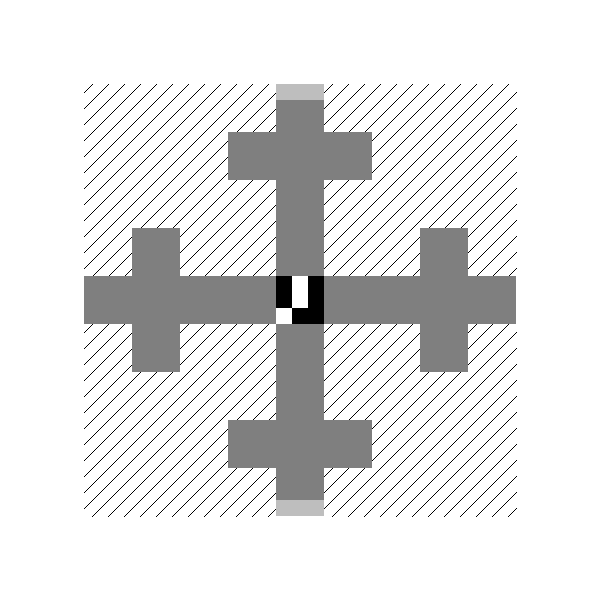
\includegraphics[width=\textwidth]{images/lycacode_layout}
    \caption{Empty}
    \label{fig:lycacode_layout}
  \end{subfigure}
  \begin{subfigure}{0.4\textwidth}
    \centering
    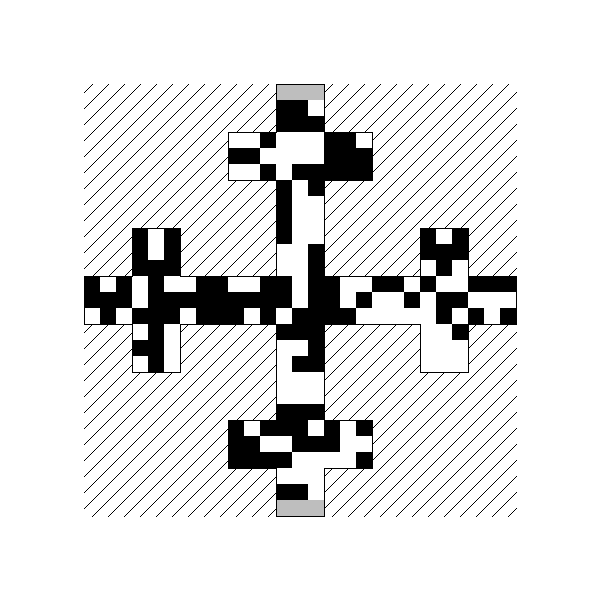
\includegraphics[width=\textwidth]{images/lycacode_data_layout}
    \caption{With data}
    \label{fig:lycacode_ex_data_layout}
  \end{subfigure}
  \caption{Lycacode layout}
\end{figure}

\subsection{Mask}
\label{ssec:lycacode_ex_mask}

As a last step, a mask is applied. The 8 masks are described in figure \ref{fig:lycacode_masks}. The best fitting one is selected based upon similar criteria as for QR-Codes\footnote{the exact criteria are defined in the python script \texttt{lycacode\_gen.py}}. Once applied to the data bits, the mask's id is encoded on the 3 reserved bits at the top and bottom of the code.

The purpose of masking in this context is purely aesthetical. It is a mean to avoid unpleasant visual patterns in the final code.

\begin{figure}[H]
  \centering
  \begin{subfigure}{0.4\textwidth}
    \centering
    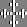
\includegraphics[width=0.4\textwidth]{images/lycacode_mask_0}
    \caption{x mod 3 = 0}
    \label{fig:lycacode_mask_0}
  \end{subfigure}
  \begin{subfigure}{0.4\textwidth}
    \centering
    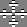
\includegraphics[width=0.4\textwidth]{images/lycacode_mask_1}
    \caption{y mod 3 = 0}
    \label{fig:lycacode_mask_1}
  \end{subfigure}
  \begin{subfigure}{0.4\textwidth}
    \centering
    
\includegraphics[width=0.4\textwidth]{images/lycacode_mask_2}
    \caption{(x+y) mod 3 = 0}
    \label{fig:lycacode_mask_2}
  \end{subfigure}
  \begin{subfigure}{0.4\textwidth}
    \centering
    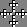
\includegraphics[width=0.4\textwidth]{images/lycacode_mask_3}
    \caption{(x mod 3)*(y mod 3) = 0}
    \label{fig:lycacode_mask_3}
  \end{subfigure}
  \begin{subfigure}{0.4\textwidth}
    \centering
    
\includegraphics[width=0.4\textwidth]{images/lycacode_mask_4}
    \caption{(y//3+x//3) mod 2 = 0}
    \label{fig:lycacode_mask_4}
  \end{subfigure}
  \begin{subfigure}{0.4\textwidth}
    \centering
    
\includegraphics[width=0.4\textwidth]{images/lycacode_mask_5}
    \caption{[(y mod 3)-1]*[(x mod 3)-(y mod 3)-2]*[(y mod 3)-(x mod 3)-2] = 0}
    \label{fig:lycacode_mask_5}
  \end{subfigure}
  \begin{subfigure}{0.4\textwidth}
    \centering
    
\includegraphics[width=0.4\textwidth]{images/lycacode_mask_6}
    \caption{(|13-x|+|13-y|) mod 3 = 1}
    \label{fig:lycacode_mask_6}
  \end{subfigure}
  \begin{subfigure}{0.4\textwidth}
    \centering
    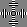
\includegraphics[width=0.4\textwidth]{images/lycacode_mask_7}
    \caption{[1-(x mod 2) + max(0, |13-y|-|13-x|)] * [1-(y mod 2) + max(0,|13-x|-|13-y|)] = 0}
    \label{fig:lycacode_mask_7}
  \end{subfigure}
  \caption{Lycacode masks}
  \label{fig:lycacode_masks}
\end{figure}

Note: "//" is integer division

For our example, the best mask is mask 3. The final binary matrix is shown in figure \ref{fig:lycacode_ex_final_mat}.

\begin{figure}[H]
  \centering
  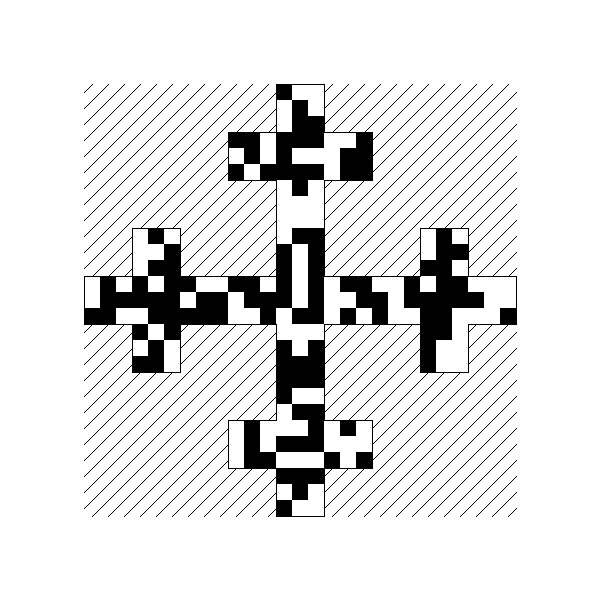
\includegraphics[width=0.5\textwidth]{images/lycacode_ex_final_mat}
  \caption{Lycacode example: masked matrix}
  \label{fig:lycacode_ex_final_mat}
\end{figure}

Finally, the matrix is converted to white dots (for 1s) on the red trefoil cross shown in figure \ref{fig:lycacode_cross}, giving the final code in figure \ref{fig:lycacode_ex_final}.

\begin{figure}[H]
  \centering
  
\includegraphics[width=0.5\textwidth]{images/lycacode_ex_final}
  \caption{Lycacode example: final code}
  \label{fig:lycacode_ex_final}
\end{figure}

The external square is used to detect the code and to correct perspective.
Its position and dimensions, which have been chosen quite arbitrarily, are visualized on figure \ref{fig:lycacode_frame}. In fact, only the position and size of the inner border is relevant in the decoding process.

\begin{figure}[H]
  \centering
  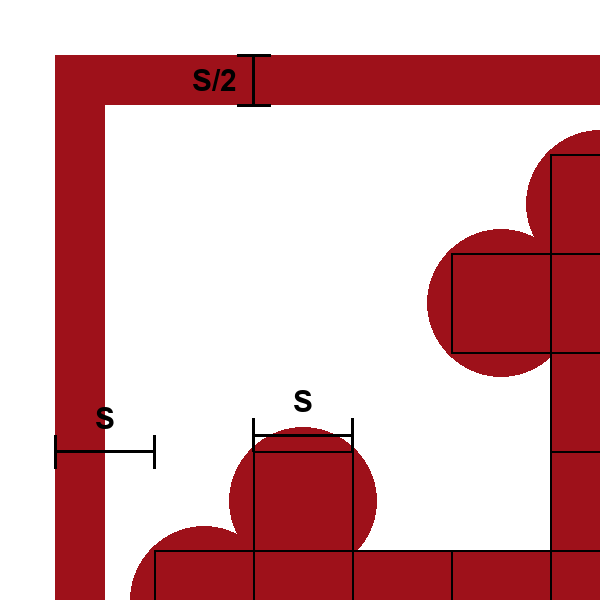
\includegraphics[width=0.5\textwidth]{images/lycacode_frame}
  \caption{Lycacode frame dimensions}
  \label{fig:lycacode_frame}
\end{figure}


  \chapter{Conclusion}
\label{chap:conclusion}

We have seen how engineers such as Woodland and Silver have built the basis for a barcode system that optimises many processes, and how these barcodes provide an easy, fast and reliable way of encoding data. These values, ease of use, speed and reliability, are most certainly what the development of new technologies is all about.
The sheer number of barcodes currently in use around the world is proof of their ingenuity.
Following the same success, QR-Codes conquered the world and became part of our daily lives as we encounter them everywhere.

Because they have become standard elements in our society, they are often disregarded and wrapped in mystery, like magical tags instantly recognizable by our devices. This work is obviously not an exhaustive list of all codes that exist. Many other types can be commonly found, such as PDF-417 or Aztec codes, both of which also use the Reed-Solomon algorithm for error-correction, or Postnet, a specialized type of barcodes used by the United States Postal Service.

The Lycacode described in \autoref{chap:custom_code} was primarily designed for education purposes, as a way to put in practice the formerly explained principles, but could well have a real application in the Collège.

  \chapter{Personal review}
\label{chap:review}

My interest for computers and programming has led me to choose this topic for my work and it is not a choice I regret.

QR-Codes were a subject I personally wanted to understand for some time but never got round to it. Having the possibility to use my knowledge in Python to apply what I had researched was also very satisfying and self-rewarding. I hope I succeeded in trying to explain the inner workings and principles making these great inventions possible. I appreciated the great freedom both on the subject's choice and the realization. Apart from learning about barcodes and QR-Codes, I have also had the opportunity to put to use my English language skills.
Using \LaTeX\  helped practising problem solving as many things can be done in multiple ways and I needed to find the best or easiest method, especially regarding tables.

The Python scripts also represent a great part of this work. While not perfect implementations, they offer a better understanding of the sometimes abstract concepts discussed and allow the generation steps to be visualized personally, using any value.

Overall, I am pleased with the fruit of my research and understanding. My only regret would be that I have not yet been able to fully understand the intricacies of Reed-Solomon codes, but I hope that one day I will.

Finally, I would like to thank Mr. Erspamer for his availability, his support and his insightful feedbacks. I must also credit my brother, who allowed me to obtain some documents such as the ISO standards\cite{ISO16388}\cite{ISO18004} and who helped with the printing of my work.


  %https://tex.stackexchange.com/a/98995
\cleardoublepage

\phantomsection

\addcontentsline{toc}{chapter}{Bibliography}

%\bibliographystyle{abbrv}

\printbibliography

  \appendix

\chapter{Python code base display module}
\label{app:base_py}

\textbf{\emph{All figures, \LaTeX\  and Python files are available on the dedicated \hreffn{https://github.com/LordBaryhobal/5D\_Heredero\_Louis\_TM2022}{GitHub repository}}}

\vspace{12pt}

This module is used by the other generator scripts to display codes.

\begin{tcolorbox}[breakable,colback=white,title=base.py]
\begin{minted}{python}
#!/usr/bin/env python
# -*- coding: utf-8 -*-
"""
This module provides a base class to display codes and enable saving

(C) 2022 Louis Heredero  louis.heredero@edu.vs.ch
"""

import pygame

class Base:
  def __init__(self, width, height, caption):
      pygame.init()

      pygame.display.set_caption(caption)
      self.w = pygame.display.set_mode([width, height])

      self.controls([
          "CTRL + S: save as",
          "ESC: quit"
      ])

  def controls(self, controls, margin=2):
      longest = max(list(map(len, controls))+[10])
      print("┌─" + "─"*(longest+margin) + "─┐")

      _ = "\x1b[1;4mControls:\x1b[0m"
      _ += " "*(longest+margin-9)
      print(f"│ " + _ + " │")
      for c in controls:
          print("│ " + " "*margin + c.ljust(longest) + " │")
      print("└─" + "─"*(longest+margin) + "─┘")

  def main(self):
      pygame.display.flip()

      stop = False
      while not stop:
          event = pygame.event.wait()
          # ESC or close button -> quit
          if event.type == pygame.QUIT:
              stop = True

          elif event.type == pygame.KEYDOWN:
              if event.key == pygame.K_ESCAPE:
                  stop = True

              # CTRL+S -> save image
              elif event.key == pygame.K_s and \
                   event.mod & pygame.KMOD_CTRL:
                  self.save()

  def save(self):
      path = input("Save as: ")
      pygame.image.save(self.w, path)
\end{minted}
\end{tcolorbox}

\chapter{Code 39 python implementation}
\label{app:code39_py}

\begin{tcolorbox}[breakable,colback=white,title=code39.py]
\begin{minted}{python}
#!/usr/bin/env python
# -*- coding: utf-8 -*-
"""
This module can generate Code-39 barcodes

(C) 2022 Louis Heredero  louis.heredero@edu.vs.ch
"""

import pygame

code39_dict = {
    "A": "100001001", "B": "001001001",
    "C": "101001000", "D": "000011001",
    "E": "100011000", "F": "001011000",
    "G": "000001101", "H": "100001100",
    "I": "001001100", "J": "000011100",
    "K": "100000011", "L": "001000011",
    "M": "101000010", "N": "000010011",
    "O": "100010010", "P": "001010010",
    "Q": "000000111", "R": "100000110",
    "S": "001000110", "T": "000010110",
    "U": "110000001", "V": "011000001",
    "W": "111000000", "X": "010010001",
    "Y": "110010000", "Z": "011010000",
    "0": "000110100", "1": "100100001",
    "2": "001100001", "3": "101100000",
    "4": "000110001", "5": "100110000",
    "6": "001110000", "7": "000100101",
    "8": "100100100", "9": "001100100",
    " ": "011000100", "-": "010000101",
    "$": "010101000", "%": "000101010",
    ".": "110000100", "/": "010100010",
    "+": "010001010", "*": "010010100"
}

def code39(text):
    text = text.upper()
    text = list(map(lambda c: code39_dict[c], text))
    return "0".join(text)

def draw_barcode(barcode, win):
    barcode = list(map(int, barcode))
    width = win.get_width()*0.8
    height = win.get_height()*0.5
    thicks = sum(barcode)
    thins = len(barcode)-thicks
    bar_w = width/(thicks*2+thins)

    win.fill((255,255,255))
    x = win.get_width()*0.1
    y = win.get_height()*0.25

    for i, c in enumerate(barcode):
        w = 2*bar_w if c else bar_w
        if i%2 == 0:
            pygame.draw.rect(win, (0,0,0), [x, y, w, height])

        x += w

if __name__ == "__main__":
    import base

    b = base.Base(800, 500, "Code-39 barcode generator")

    barcode = code39("*CODE-39*")
    draw_barcode(barcode, b.w)

    b.main()
\end{minted}
\end{tcolorbox}

\chapter{EAN python implementation}
\label{app:ean_py}

\begin{tcolorbox}[breakable,colback=white,title=ean.py]
\begin{minted}{python}
#!/usr/bin/env python
# -*- coding: utf-8 -*-
"""
This module can generate EAN-8 and EAN-13 barcodes

(C) 2022 Louis Heredero  louis.heredero@edu.vs.ch
"""

import pygame

A = [
    0b0001101,
    0b0011001,
    0b0010011,
    0b0111101,
    0b0100011,
    0b0110001,
    0b0101111,
    0b0111011,
    0b0110111,
    0b0001011
]

# XOR 0b1111111
C = list(map(lambda a: a^127, A))

# Reverse bit order
B = list(map(lambda c: int(f"{c:07b}"[::-1],2), C))

ean13_patterns = [
    "AAAAAA",
    "AABABB",
    "AABBAB",
    "AABBBA",
    "ABAABB",
    "ABBAAB",
    "ABBBAA",
    "ABABAB",
    "ABABBA",
    "ABBABA"
]

def bin_list(n):
    return list(map(int,f"{n:07b}"))

def luhn(digits):
    checksum = sum([
        digits[-i-1]*(3-i%2*2)
        for i in range(len(digits))
    ])
    ctrl_key = 10 - checksum%10
    if ctrl_key == 10:
        ctrl_key = 0

    return ctrl_key

def ean8(digits):
    digits.append(luhn(digits))
    elmts = []

    elmts += [1,0,1] #delimiter
    for digit in digits[:4]:
        elmts += bin_list(A[digit])

    elmts += [0,1,0,1,0] #middle delimiter
    for digit in digits[4:]:
        elmts += bin_list(C[digit])

    elmts += [1,0,1] #delimiter
    return elmts

def ean13(digits):
    pattern = ean13_patterns[digits[0]]
    digits.append(luhn(digits))
    elmts = []

    elmts += [1,0,1] #delimiter
    for d in range(1,7):
        _ = A if pattern[d-1] == "A" else B
        digit = digits[d]
        elmts += bin_list(_[digit])

    elmts += [0,1,0,1,0] #middle delimiter
    for digit in digits[7:]:
        elmts += bin_list(C[digit])

    elmts += [1,0,1] #delimiter
    return elmts

def draw_barcode(barcode, win):
    width = win.get_width()*0.8
    height = win.get_height()*0.5
    bar_w = width/len(barcode)
    rnd_bar_w = round(bar_w)

    win.fill((255,255,255))
    x = win.get_width()*0.1
    y = win.get_height()*0.25

    for c in barcode:
        if c:
            pygame.draw.rect(win, (0,0,0), [x, y, rnd_bar_w, height])

        x += bar_w

if __name__ == "__main__":
    import base

    b = base.Base(800, 500, "EAN-8 / EAN-13 barcode generator")

    #barcode = ean8([8,4,2,7,3,7,2])
    barcode = ean13([9,7,8,2,9,4,0,6,2,1,0,5])

    draw_barcode(barcode, b.w)

    b.main()
\end{minted}
\end{tcolorbox}

\chapter{QR-Code tables}
\label{app:qr_tabs}

\def\arraystretch{1.2}
\begin{table}[H]
  \centering
  \begin{tabu}{|[2pt]c|c|[2pt]c|c|[2pt]c|c|[2pt]}
    \tabucline[2pt]{-}
    Index & Char & Index & Char & Index & Char \\
    \hline
    0 & 0 & 15 & F & 30 & U \\
    \hline
    1 & 1 & 16 & G & 31 & V \\
    \hline
    2 & 2 & 17 & H & 32 & W \\
    \hline
    3 & 3 & 18 & I & 33 & X \\
    \hline
    4 & 4 & 19 & J & 34 & Y \\
    \hline
    5 & 5 & 20 & K & 35 & Z \\
    \hline
    6 & 6 & 21 & L & 36 & \emph{space} \\
    \hline
    7 & 7 & 22 & M & 37 & \$ \\
    \hline
    8 & 8 & 23 & N & 38 & \% \\
    \hline
    9 & 9 & 24 & O & 39 & * \\
    \hline
    10 & A & 25 & P & 40 & + \\
    \hline
    11 & B & 26 & Q & 41 & - \\
    \hline
    12 & C & 27 & R & 42 & . \\
    \hline
    13 & D & 28 & S & 43 & / \\
    \hline
    14 & E & 29 & T & 44 & : \\
    \tabucline[2pt]{-}
  \end{tabu}
  \caption{List of alphanumerical characters}
  \label{tab:qr_alphanum}
\end{table}
\def\arraystretch{1}

\def\arraystretch{1.2}
\begin{center}
  \begin{longtabu}{|[2pt]c|c|c:c:c:c|[2pt]}
    \caption{Version capacities}
    \label{tab:qr_versions}\\
    \tabucline[2pt]{-}
    Version & Correction level & Numerical & Alphanumerical & Byte & Kanji \\
    \tabucline[2pt]{-}
    \endfirsthead
    \multicolumn{6}{r}{\emph{Continued from last page}}\\
    \endhead
    \multicolumn{6}{r}{\emph{Continued on next page}}\\
    \endfoot
    \tabucline[2pt]{-}
    \endlastfoot
    \multirow{4}{*}{ 1} & L &   41 &   25 &   17 &   10 \\*
                        & M &   34 &   20 &   14 &    8 \\*
                        & Q &   27 &   16 &   11 &    7 \\*
                        & H &   17 &   10 &    7 &    4 \\
    \hline
    \multirow{4}{*}{ 2} & L &   77 &   47 &   32 &   20 \\*
                        & M &   63 &   38 &   26 &   16 \\*
                        & Q &   48 &   29 &   20 &   12 \\*
                        & H &   34 &   20 &   14 &    8 \\
    \hline
    \multirow{4}{*}{ 3} & L &  127 &   77 &   53 &   32 \\*
                        & M &  101 &   61 &   42 &   26 \\*
                        & Q &   77 &   47 &   32 &   20 \\*
                        & H &   58 &   35 &   24 &   15 \\
    \hline
    \multirow{4}{*}{ 4} & L &  187 &  114 &   78 &   48 \\*
                        & M &  149 &   90 &   62 &   38 \\*
                        & Q &  111 &   67 &   46 &   28 \\*
                        & H &   82 &   50 &   34 &   21 \\
    \hline
    \multirow{4}{*}{ 5} & L &  255 &  154 &  106 &   65 \\*
                        & M &  202 &  122 &   84 &   52 \\*
                        & Q &  144 &   87 &   60 &   37 \\*
                        & H &  106 &   64 &   44 &   27 \\
    \hline
    \multirow{4}{*}{ 6} & L &  322 &  195 &  134 &   82 \\*
                        & M &  255 &  154 &  106 &   65 \\*
                        & Q &  178 &  108 &   74 &   45 \\*
                        & H &  139 &   84 &   58 &   36 \\
    \hline
    \multirow{4}{*}{ 7} & L &  370 &  224 &  154 &   95 \\*
                        & M &  293 &  178 &  122 &   75 \\*
                        & Q &  207 &  125 &   86 &   53 \\*
                        & H &  154 &   93 &   64 &   39 \\
    \hline
    \multirow{4}{*}{ 8} & L &  461 &  279 &  192 &  118 \\*
                        & M &  365 &  221 &  152 &   93 \\*
                        & Q &  259 &  157 &  108 &   66 \\*
                        & H &  202 &  122 &   84 &   52 \\
    \hline
    \multirow{4}{*}{ 9} & L &  552 &  335 &  230 &  141 \\*
                        & M &  432 &  262 &  180 &  111 \\*
                        & Q &  312 &  189 &  130 &   80 \\*
                        & H &  235 &  143 &   98 &   60 \\
    \hline
    \multirow{4}{*}{10} & L &  652 &  395 &  271 &  167 \\*
                        & M &  513 &  311 &  213 &  131 \\*
                        & Q &  364 &  221 &  151 &   93 \\*
                        & H &  288 &  174 &  119 &   74 \\
    \hline
    \multirow{4}{*}{11} & L &  772 &  468 &  321 &  198 \\*
                        & M &  604 &  366 &  251 &  155 \\*
                        & Q &  427 &  259 &  177 &  109 \\*
                        & H &  331 &  200 &  137 &   85 \\
    \hline
    \multirow{4}{*}{12} & L &  883 &  535 &  367 &  226 \\*
                        & M &  691 &  419 &  287 &  177 \\*
                        & Q &  489 &  296 &  203 &  125 \\*
                        & H &  374 &  227 &  155 &   96 \\
    \hline
    \multirow{4}{*}{13} & L & 1022 &  619 &  425 &  262 \\*
                        & M &  796 &  483 &  331 &  204 \\*
                        & Q &  580 &  352 &  241 &  149 \\*
                        & H &  427 &  259 &  177 &  109 \\
    \hline
    \multirow{4}{*}{14} & L & 1101 &  667 &  458 &  282 \\*
                        & M &  871 &  528 &  362 &  223 \\*
                        & Q &  621 &  376 &  258 &  159 \\*
                        & H &  468 &  283 &  194 &  120 \\
    \hline
    \multirow{4}{*}{15} & L & 1250 &  758 &  520 &  320 \\*
                        & M &  991 &  600 &  412 &  254 \\*
                        & Q &  703 &  426 &  292 &  180 \\*
                        & H &  530 &  321 &  220 &  136 \\
    \hline
    \multirow{4}{*}{16} & L & 1408 &  854 &  586 &  361 \\*
                        & M & 1082 &  656 &  450 &  277 \\*
                        & Q &  775 &  470 &  322 &  198 \\*
                        & H &  602 &  365 &  250 &  154 \\
    \hline
    \multirow{4}{*}{17} & L & 1548 &  938 &  644 &  397 \\*
                        & M & 1212 &  734 &  504 &  310 \\*
                        & Q &  876 &  531 &  364 &  224 \\*
                        & H &  674 &  408 &  280 &  173 \\
    \hline
    \multirow{4}{*}{18} & L & 1725 & 1046 &  718 &  442 \\*
                        & M & 1346 &  816 &  560 &  345 \\*
                        & Q &  948 &  574 &  394 &  243 \\*
                        & H &  746 &  452 &  310 &  191 \\
    \hline
    \multirow{4}{*}{19} & L & 1903 & 1153 &  792 &  488 \\*
                        & M & 1500 &  909 &  624 &  384 \\*
                        & Q & 1063 &  644 &  442 &  272 \\*
                        & H &  813 &  493 &  338 &  208 \\
    \hline
    \multirow{4}{*}{20} & L & 2061 & 1249 &  858 &  528 \\*
                        & M & 1600 &  970 &  666 &  410 \\*
                        & Q & 1159 &  702 &  482 &  297 \\*
                        & H &  919 &  557 &  382 &  235 \\
    \hline
    \multirow{4}{*}{21} & L & 2232 & 1352 &  929 &  572 \\*
                        & M & 1708 & 1035 &  711 &  438 \\*
                        & Q & 1224 &  742 &  509 &  314 \\*
                        & H &  969 &  587 &  403 &  248 \\
    \hline
    \multirow{4}{*}{22} & L & 2409 & 1460 & 1003 &  618 \\*
                        & M & 1872 & 1134 &  779 &  480 \\*
                        & Q & 1358 &  823 &  565 &  348 \\*
                        & H & 1056 &  640 &  439 &  270 \\
    \hline
    \multirow{4}{*}{23} & L & 2620 & 1588 & 1091 &  672 \\*
                        & M & 2059 & 1248 &  857 &  528 \\*
                        & Q & 1468 &  890 &  611 &  376 \\*
                        & H & 1108 &  672 &  461 &  284 \\
    \hline
    \multirow{4}{*}{24} & L & 2812 & 1704 & 1171 &  721 \\*
                        & M & 2188 & 1326 &  911 &  561 \\*
                        & Q & 1588 &  963 &  661 &  407 \\*
                        & H & 1228 &  744 &  511 &  315 \\
    \hline
    \multirow{4}{*}{25} & L & 3057 & 1853 & 1273 &  784 \\*
                        & M & 2395 & 1451 &  997 &  614 \\*
                        & Q & 1718 & 1041 &  715 &  440 \\*
                        & H & 1286 &  779 &  535 &  330 \\
    \hline
    \multirow{4}{*}{26} & L & 3283 & 1990 & 1367 &  842 \\*
                        & M & 2544 & 1542 & 1059 &  652 \\*
                        & Q & 1804 & 1094 &  751 &  462 \\*
                        & H & 1425 &  864 &  593 &  365 \\
    \hline
    \multirow{4}{*}{27} & L & 3517 & 2132 & 1465 &  902 \\*
                        & M & 2701 & 1637 & 1125 &  692 \\*
                        & Q & 1933 & 1172 &  805 &  496 \\*
                        & H & 1501 &  910 &  625 &  385 \\
    \hline
    \multirow{4}{*}{28} & L & 3669 & 2223 & 1528 &  940 \\*
                        & M & 2857 & 1732 & 1190 &  732 \\*
                        & Q & 2085 & 1263 &  868 &  534 \\*
                        & H & 1581 &  958 &  658 &  405 \\
    \hline
    \multirow{4}{*}{29} & L & 3909 & 2369 & 1628 & 1002 \\*
                        & M & 3035 & 1839 & 1264 &  778 \\*
                        & Q & 2181 & 1322 &  908 &  559 \\*
                        & H & 1677 & 1016 &  698 &  430 \\
    \hline
    \multirow{4}{*}{30} & L & 4158 & 2520 & 1732 & 1066 \\*
                        & M & 3289 & 1994 & 1370 &  843 \\*
                        & Q & 2358 & 1429 &  982 &  604 \\*
                        & H & 1782 & 1080 &  742 &  457 \\
    \hline
    \multirow{4}{*}{31} & L & 4417 & 2677 & 1840 & 1132 \\*
                        & M & 3486 & 2113 & 1452 &  894 \\*
                        & Q & 2473 & 1499 & 1030 &  634 \\*
                        & H & 1897 & 1150 &  790 &  486 \\
    \hline
    \multirow{4}{*}{32} & L & 4686 & 2840 & 1952 & 1201 \\*
                        & M & 3693 & 2238 & 1538 &  947 \\*
                        & Q & 2670 & 1618 & 1112 &  684 \\*
                        & H & 2022 & 1226 &  842 &  518 \\
    \hline
    \multirow{4}{*}{33} & L & 4965 & 3009 & 2068 & 1273 \\*
                        & M & 3909 & 2369 & 1628 & 1002 \\*
                        & Q & 2805 & 1700 & 1168 &  719 \\*
                        & H & 2157 & 1307 &  898 &  553 \\
    \hline
    \multirow{4}{*}{34} & L & 5253 & 3183 & 2188 & 1347 \\*
                        & M & 4134 & 2506 & 1722 & 1060 \\*
                        & Q & 2949 & 1787 & 1228 &  756 \\*
                        & H & 2301 & 1394 &  958 &  590 \\
    \hline
    \multirow{4}{*}{35} & L & 5529 & 3351 & 2303 & 1417 \\*
                        & M & 4343 & 2632 & 1809 & 1113 \\*
                        & Q & 3081 & 1867 & 1283 &  790 \\*
                        & H & 2361 & 1431 &  983 &  605 \\
    \hline
    \multirow{4}{*}{36} & L & 5836 & 3537 & 2431 & 1496 \\*
                        & M & 4588 & 2780 & 1911 & 1176 \\*
                        & Q & 3244 & 1966 & 1351 &  832 \\*
                        & H & 2524 & 1530 & 1051 &  647 \\
    \hline
    \multirow{4}{*}{37} & L & 6153 & 3729 & 2563 & 1577 \\*
                        & M & 4775 & 2894 & 1989 & 1224 \\*
                        & Q & 3417 & 2071 & 1423 &  876 \\*
                        & H & 2625 & 1591 & 1093 &  673 \\
    \hline
    \multirow{4}{*}{38} & L & 6479 & 3927 & 2699 & 1661 \\*
                        & M & 5039 & 3054 & 2099 & 1292 \\*
                        & Q & 3599 & 2181 & 1499 &  923 \\*
                        & H & 2735 & 1658 & 1139 &  701 \\
    \hline
    \multirow{4}{*}{39} & L & 6743 & 4087 & 2809 & 1729 \\*
                        & M & 5313 & 3220 & 2213 & 1362 \\*
                        & Q & 3791 & 2298 & 1579 &  972 \\*
                        & H & 2927 & 1774 & 1219 &  750 \\
    \hline
    \multirow{4}{*}{40} & L & 7089 & 4296 & 2953 & 1817 \\*
                        & M & 5596 & 3391 & 2331 & 1435 \\*
                        & Q & 3993 & 2420 & 1663 & 1024 \\*
                        & H & 3057 & 1852 & 1273 &  784 \\
    \hline
  \end{longtabu}
\end{center}
\def\arraystretch{1}


% Rotated headers
% https://tex.stackexchange.com/a/98439
\chapter{Error detection and correction}
\label{chap:err_corr}

This chapter introduces two methods to create self-correcting messages: Hamming codes and Reed-Solomon codes. The former is based on parity bits while the latter takes advantage of advanced mathematical properties of modular arithmetic and polynomials.

\section{Hamming Codes}
\label{sec:hamming}

When working with binary data, one way of checking if a received message is corrupted or not is to add a parity bit. The parity of a binary number is even if it has an even number of 1s and odd otherwise. A parity check bit is added such that the total parity of the number is even, i.e. 0 if it is already even, 1 otherwise.

\def\arraystretch{1.2}
\begin{center}
  \begin{tabular}{|c|c|c|c|c||c|c}
    \multicolumn{5}{c}{} & \multicolumn{1}{c}{parity bit} & \\
    \cline{1-6}
    bit 1 & bit 2 & bit 3 & bit 4 & bit 5 & bit 6 & \multirow{2}{*}{parity: even} \\
    \cline{1-6}
    1 & 1 & 0 & 0 & 1 & 1 & \\
    \cline{1-6}
  \end{tabular}
\end{center}
\def\arraystretch{1}

With this, a single bit error (that is, one bit is wrong) is easy to detect because the parity of the message becomes odd.

\def\arraystretch{1.2}
\begin{center}
  \begin{tabular}{|c|c|c|c|c|c|c}
    \cline{1-6}
    bit 1 & bit 2 & bit 3 & bit 4 & bit 5 & bit 6 & \multirow{2}{*}{parity: odd} \\
    \cline{1-6}
    1 & 1 & \textbf{1} & 0 & 1 & 1 & \\
    \cline{1-6}
  \end{tabular}
\end{center}
\def\arraystretch{1}

However, a single parity bit doesn't provide enough information to allow locating the error or detecting multiple errors, because an even number of errors would keep an even parity overall.

\def\arraystretch{1.2}
\begin{center}
  \begin{tabular}{|c|c|c|c|c|c|c}
    \cline{1-6}
    bit 1 & bit 2 & bit 3 & bit 4 & bit 5 & bit 6 & \multirow{2}{*}{parity: even} \\
    \cline{1-6}
    1 & 1 & \textbf{1} & 0 & \textbf{0} & 1 & \\
    \cline{1-6}
  \end{tabular}
\end{center}
\def\arraystretch{1}

Hamming codes are a kind of parity check codes.
Instead of using only one parity bit however, they include several so that locating becomes possible, as well as detecting (not always) multiple errors.

When creating a Hamming code from a message, data first has to be split into blocks of a given size. For each block a certain number of parity bits is assigned. These two variables (blocksize and number of parity bits) determine the type of Hamming code.
For example a Hamming code with 3 parity bits will form 7-bit blocks, meaning each block can hold 4 data bits. It can thus be called Hamming(7, 4).

Smaller blocksizes allow more errors to be corrected, because each block can correct one error, but have a lower data density\footnote{data density is the ratio of data bits over blocksize}. On the other hand, larger blocksizes allow less errors to be corrected but have a higher data density.

Hamming codes are created in such a way that when a bit is flipped, the parity bits indicate exactly where the error occured. For that, each position in the code which is a power of two is a parity bits. Then, each parity bit covers the parity of all bits at positions containing its power in their binary representation. For example, the parity bit at position 4 (0b\ul{1}00) covers bits 5 (0b\ul{1}01), 6 (0b\ul{1}10), 7 (0b\ul{1}11), 12 (0b1\ul{1}00), 13 (0b1\ul{1}01), 14 (0b1\ul{1}10), 15 (0b1\ul{1}11), ...

Table \ref{tab:hamming_struct} taken from \citetitle{hamming_wiki}\cite{hamming_wiki} offers a good visual representation of this structure:

\def\arraystretch{1.5}
\begin{table}[H]
  \centering
  \resizebox{\textwidth}{!}{
  \begin{tabular}{|c|c|c|c|c|c|c|c|c|c|c|c|c|c|c|c|c|}
    \hline
    \rowcolor{tabgrey} \multicolumn{2}{|c|}{Bit position} & 1 & 2 & 3 & 4 & 5 & 6 & 7 & 8 & 9 & 10 & 11 & 12 & 13 & 14 & 15 \\
    \hhline{-|-|-|-|-|-|-|-|-|-|-|-|-|-|-|-|-|}
    \rowcolor{tabgrey} \multicolumn{2}{|c|}{Encoded data bits} & \cellcolor{paritybg} p1 & \cellcolor{paritybg} p2 & d1 & \cellcolor{paritybg} p4 & d2 & d3 & d4 & \cellcolor{paritybg} p8 & d5 & d6 & d7 & d8 & d9 & d10 & d11 \\
    \hhline{-|-|-|-|-|-|-|-|-|-|-|-|-|-|-|-|-|}
    \multirow{4}{*}{\shortstack{Parity\\ bit\\ coverage}} & \cellcolor{paritybg} p1 & \tick & & \tick & & \tick & & \tick & & \tick & & \tick & & \tick & & \tick \\
    \hhline{~|-|-|-|-|-|-|-|-|-|-|-|-|-|-|-|-|}
     & \cellcolor{paritybg} p2 & & \tick & \tick & & & \tick & \tick & & & \tick & \tick & & & \tick & \tick \\
    \hhline{~|-|-|-|-|-|-|-|-|-|-|-|-|-|-|-|-|}
      & \cellcolor{paritybg} p4 & & & & \tick & \tick & \tick & \tick & & & & & \tick & \tick & \tick & \tick \\
    \hhline{~|-|-|-|-|-|-|-|-|-|-|-|-|-|-|-|-|}
      & \cellcolor{paritybg} p8 & & & & & & & & \tick & \tick & \tick & \tick & \tick & \tick & \tick & \tick \\
    \hline
  \end{tabular}}
  \caption{Hamming code structure}
  \label{tab:hamming_struct}
\end{table}
\def\arraystretch{1}

Here we can see that each data bit (d1, d2, d3, ...) is covered by a unique set of parity bits.

\pagebreak

Let's create a Hamming(15, 11) code for the message \texttt{11101100010}.
The first step is to lay out the bits in table \ref{tab:hamming_struct} like so:

\def\arraystretch{1.5}
\begin{table}[H]
  \centering
  \resizebox{\textwidth}{!}{
  \begin{tabular}{|c|c|c|c|c|c|c|c|c|c|c|c|c|c|c|c|c|}
    \hline
    \rowcolor{tabgrey} \multicolumn{2}{|c|}{Bit position} & 1 & 2 & 3 & 4 & 5 & 6 & 7 & 8 & 9 & 10 & 11 & 12 & 13 & 14 & 15 \\
    \hline
    \multicolumn{2}{|c|}{\cellcolor{tabgrey} Encoded data bits} & p1 & p2 & 1 & p4 & 1 & 1 & 0 & p8 & 1 & 1 & 0 & 0 & 0 & 1 & 0 \\
    \hline
    \multirow{4}{*}{\shortstack{Parity\\ bit\\ coverage}} & \cellcolor{paritybg} p1 & - & & \tick & & \tick & & \cross & & \tick & & \cross & & \cross & & \cross \\
    \hhline{~|-|-|-|-|-|-|-|-|-|-|-|-|-|-|-|-|}
     & \cellcolor{paritybg} p2 & & - & \tick & & & \tick & \cross & & & \tick & \cross & & & \tick & \cross \\
    \hhline{~|-|-|-|-|-|-|-|-|-|-|-|-|-|-|-|-|}
      & \cellcolor{paritybg} p4 & & & & - & \tick & \tick & \cross & & & & & \cross & \cross & \tick & \cross \\
    \hhline{~|-|-|-|-|-|-|-|-|-|-|-|-|-|-|-|-|}
      & \cellcolor{paritybg} p8 & & & & & & & & - & \tick & \tick & \cross & \cross & \cross & \tick & \cross \\
    \hline
  \end{tabular}}

  \medskip

  \begin{tabular}{|c|c|c|c|}
    \hline
    \rowcolor{tabgrey} Parity bit & Covered 1s & Parity of covered bits & Value \\
    \hline
    p1 & 3 & odd & 1 \\
    \hline
    p2 & 4 & even & 0 \\
    \hline
    p4 & 3 & odd & 1 \\
    \hline
    p8 & 3 & odd & 1 \\
    \hline
  \end{tabular}
  \caption{Hamming code example}
  \label{tab:hamming_ex}
\end{table}
\def\arraystretch{1}

Placing the parity bits in their relevant positions, we get the hamming code \texttt{101111011100010}.

%\bigskip

To illustrate the decoding process, let's alter bit 11 and change it to a 1.
Now, recalculating the parity bits and comparing the results with the received message, we can find the location of the error.

\def\arraystretch{1.5}
\begin{table}[H]
  \centering
  \resizebox{\textwidth}{!}{
  \begin{tabular}{|c|c|c|c|c|c|c|c|c|c|c|c|c|c|c|c|c|}
    \hline
    \rowcolor{tabgrey} \multicolumn{2}{|c|}{Bit position} & 1 & 2 & 3 & 4 & 5 & 6 & 7 & 8 & 9 & 10 & 11 & 12 & 13 & 14 & 15 \\
    \hline
    \multicolumn{2}{|c|}{\cellcolor{tabgrey} Received data bits} & 1 & 0 & 1 & 1 & 1 & 1 & 0 & 1 & 1 & 1 & \textbf{1} & 0 & 0 & 1 & 0 \\
    \hline
    \multirow{4}{*}{\shortstack{Parity\\ bit\\ coverage}} & \cellcolor{paritybg} p1 & - & & \tick & & \tick & & \cross & & \tick & & \tick & & \cross & & \cross \\
    \hhline{~|-|-|-|-|-|-|-|-|-|-|-|-|-|-|-|-|}
     & \cellcolor{paritybg} p2 & & - & \tick & & & \tick & \cross & & & \tick & \tick & & & \tick & \cross \\
    \hhline{~|-|-|-|-|-|-|-|-|-|-|-|-|-|-|-|-|}
      & \cellcolor{paritybg} p4 & & & & - & \tick & \tick & \cross & & & & & \cross & \cross & \tick & \cross \\
    \hhline{~|-|-|-|-|-|-|-|-|-|-|-|-|-|-|-|-|}
      & \cellcolor{paritybg} p8 & & & & & & & & - & \tick & \tick & \tick & \cross & \cross & \tick & \cross \\
    \hline
  \end{tabular}}

  \medskip

  \begin{tabular}{|c|c|c|c|c|}
    \hline
    \rowcolor{tabgrey} Parity bit & Covered 1s & Parity of covered bits & Value & Received value \\
    \hline
    p1 & 4 & even & 0 & 1 \\
    \hline
    p2 & 5 & odd & 1 & 0 \\
    \hline
    p4 & 3 & odd & 1 & 1 \\
    \hline
    p8 & 4 & even & 0 & 1 \\
    \hline
  \end{tabular}
  \caption{Hamming code example decoding}
  \label{tab:hamming_ex_decoding}
\end{table}
\def\arraystretch{1}

The difference (XOR) between columns "Value" and "Received value" forms the binary number \texttt{0b1101} = 11, the location of the error.

\section{Reed-Solomon algorithm}
\label{sec:reed_solomon}

The Reed-Solomon algorithm is a mathematical process allowing the decoding of a partially corrupted message. It is used in many domains for its strength and reliability, such as for spatial communication, CD/DVD players, some television broadcasts and QR-Codes.

Reed-Solomon codes were developed by Irving S. Reed and Gustave Solomon in 1960 \cite{reed_solomon}

As they rely on abstract and complex mathematical concepts, this section will not go in specific details about the actual decoding process. For curious readers, see
\citetitle{computerphile_rs}\cite{computerphile_rs} (presentation, general concept), \citetitle{reed_solomon_wiki}\cite{reed_solomon_wiki} (in depth article) and \citetitle{nasa_rs}\cite{nasa_rs} (complete manual and explanations)

\subsection{Error detection}
\label{ssec:rs_error_detection}

Before considering error correction, it is necessary to talk about error detection. Several methods have been developed for this purpose.

The most basic, as seen in \autoref{sec:hamming}, is a parity check. It consists of appending one or more "parity bits" to a binary message, such that the overall parity is known. For example, let table \ref{tab:err_det_raw} be our raw message

\def\arraystretch{1.5}
\begin{table}[H]
  \centering
  \begin{tabu}{|cccccccc|}
    \hline
    0 & 1 & 0 & 0 & 0 & 0 & 1 & 1 \\
    \hline
  \end{tabu}
  \caption{Error detection: raw message}
  \label{tab:err_det_raw}
\end{table}
\def\arraystretch{1}

The parity of this byte is odd -- because there are 3 1s -- so an additional 1 is added to the end.

In this way, if the message is corrupted -- by 1 bit maximum -- it becomes even, and we know there is an error.
Now obviously it doesn't provide any information on the exact location of the error in the message and can't detect an even number of errors.

However, this principle can be extended to include a parity bit for every byte.
If represented as a table in which each row is a byte, it can also include parity bits for each column.
Table \ref{tab:err_det_tab} is an example of such usage of parity bits. This implementation is even able to correct a single error as the row and column would be odd.

\def\arraystretch{1.4}
\begin{table}[H]
  \centering
  \begin{tabu}{|[2pt]c|cccccccc|c|[2pt]}
    \tabucline[2pt]{-}
    & bit 0 & bit 1 & bit 2 & bit 3 & bit 4 & bit 5 & bit 6 & bit 7 & parity \\
    \hline
    byte 0 & 0 & 1 & 0 & 0 & 0 & 0 & 1 & 1 & 1 \\
    byte 1 & 0 & 1 & 1 & 0 & 1 & 1 & 1 & 1 & 0 \\
    byte 2 & 0 & 1 & 1 & 0 & 0 & 1 & 0 & 0 & 1 \\
    byte 3 & 0 & 1 & 1 & 0 & 0 & 1 & 0 & 1 & 0 \\
    byte 4 & 0 & 1 & 1 & 1 & 0 & 0 & 1 & 1 & 1 \\
    \hline
    parity & 0 & 1 & 0 & 1 & 1 & 1 & 1 & 0 & 1 \\
    \tabucline[2pt]{-}
  \end{tabu}
  \caption{Error detection: bytes table parity}
  \label{tab:err_det_tab}
\end{table}
\def\arraystretch{1}

Such codes however don't provide enough error correction capability - at most 1 bit. Other methods, like the previously explained Hamming codes, allow a more efficient use of parity bits, increasing to some degree the number of fixable errors.

Reed-Solomon codes use properties of polynomials and modular arithmetic to produce more efficient and more robust correction data.

\subsection{Binary to polynomials}
\label{ssec:rs_bin_to_poly}
Instead of working directly with binary data, Reed-Solomon codes treat messages as polynomials.
These are formed from binary data as follows: each byte is converted to a decimal integer, representing coefficients of the polynomial.

For example:
\def\arraystretch{1.4}
\begin{tabu}{|[1pt]c|c|c|c|c|c|[1pt]}
  \tabucline[1pt]{-}
  raw binary & $01000011$ & $01101111$ & $01100100$ & $01100101$ & $01110011$ \\
  \hline
  decimal & $67$ & $111$ & $100$ & $101$ & $115$ \\
  \hline
  polynomial & \multicolumn{5}{c|[1pt]}{$67x^4 + 111x^3 + 100x^2 + 101x + 115$}\\
  \tabucline[1pt]{-}
\end{tabu}
\def\arraystretch{1}

\subsection{Galois Fields}
\label{ssec:rs_galois}
Since the main applications of Reed-Solomon codes are related to digital devices, it is relevant to use bits and bytes. As such, all calculations are performed in a Galois field. A Galois field is basicly a finite set of numbers on which arithmetic operations results in numbers of the set. In the case of QR-Codes, G(256) -- a Galois field of the integers 0 to 255 incl. -- is used. This means every operation between numbers results in a value between 0 and 255 incl., which is an eight-bit positive integer. In this field, addition and subtraction are equivalent and defined as the binary XOR operation. For example:

\begin{gather*}
  17 + 13 = 17 - 13 = 28 \\
  \Leftrightarrow 0\text{b}10001 \oplus 0\text{b}1101 = 0\text{b}1101 \oplus 0\text{b}10001 = 0\text{b}11100
\end{gather*}

Multiplication is more complex though. One property of this Galois field is that every number can be represented as a power of two, XOR 285.
For example:
\begin{equation*}
  \begin{split}
    2^{17} =& (\underbrace{2^8}_{256} \oplus 285) * 2^9 = 29 * 2^9 \\
         =& [\underbrace{(29 * 2^4)}_{464} \oplus 285] * 2^5 = 205 * 2^5 \\
         =& [\underbrace{(205 * 2)}_{410} \oplus 285] * 2^4 = 135 * 2^4 \\
         =& [\underbrace{(135 * 2)}_{270} \oplus 285] * 2^3 = 19 * 2^3 \\
         =& 152 \\
    \Rightarrow& \exp_2(17) = 152 \\
    \Rightarrow& \log_2(152) = 17
  \end{split}
\end{equation*}

To multiply two numbers $a$ and $b$ in the Galois field:\footnote{from now on, $\exp$ and $\log$ are assumed to be base 2} \[
  a * b = \exp(\log(a) + \log(b))
\]
which also works in regular arithmetic (in $\mathbb{N}^*_+$).

Division works similarly, but because there are no negative or fractional number in the field, the exponent is kept in the range 0-255 incl. like so: \[
  \frac{a}{b} = \exp([\log(a) - \log(b) + 255]\ mod \ 255)
\]

And powers too: \[
  a^b = \exp([\log(a) * b]\ mod\ 255)
\]

\subsection{Generating error correction}
\label{ssec:rs_gen}
To create Reed-Solomon error correction bytes, a generator polynomial $g(x)$ is needed.
This polynomial is created using equation \ref{equ:rs_gen_poly}:
\begin{equation}
  g(x) = \prod_{i=0}^{d-1} (x + 2^i)
  \label{equ:rs_gen_poly}
\end{equation}

where $d$ is one more than the degree of the polynomial, equivalent to the number of error correction bytes.

Let $m(x)$ be our message polynomial (see \autoref{ssec:rs_bin_to_poly}) and $g(x)$ the generator polynomial. The error correction polynomial $E_c(x)$ is then the remainder of the long polynomial division $m(x)/g(x)$.

Let's illustrate this by creating error correction for the string "Codes". In UTF-8, the message bytes are 67, 111, 100, 101, 115, thus $m(x) = 67x^4+ 111x^3+ 100x^2+ 101x+ 115$.
% We will take the generator polynomial of degree 3, that is: \[
%   g(x) = (x + 1)*(x + 2)*(x + 4)\\
%   = x^3 + 7x^2 + 14x + 8
% \]
We will take the generator polynomial of degree 4, that is: \[
  g(x) = (x + 1)*(x + 2)*(x + 4)*(x + 8)\\
  = x^4 + 15x^3 + 54x^2 + 120x + 64
\]

And thus (reminder that addition and subtraction in the galois field is the binary XOR operation):
\begin{comment}
\[
  \def\arraystretch{1.5}
  \begin{array}{rrrrrrrrrrrrr}
     67 &  111 &  100 & 101 &  115 &    0 &    0 &    0 &\divline{}&   1 &   7 & 14 &  8 \\
    \cline{9-13}
    -67 & -212 & -181 & -34 &      &      &      &      &       67 & 187 & 215 & 84 & 77 \\
    \cline{1-4}
        &  187 &  209 &  71 &  115 &      &      &      &          &     &     &    & \\
        & -187 &   -6 & -12 & -177 &      &      &      &          &     &     &    & \\
    \cline{2-5}
        &      &  215 &  75 &  194 &    0 &      &      &          &     &     &    & \\
        &      & -215 & -31 &  -52 & -246 &      &      &          &     &     &    & \\
    \cline{3-6}
        &      &      &  84 &  252 &  246 &    0 &      &          &     &     &    & \\
        &      &      & -84 & -177 & -127 & -154 &      &          &     &     &    & \\
    \cline{4-7}
        &      &      &     &   77 &  137 &  154 &    0 &          &     &     &    & \\
        &      &      &     &  -77 & -254 & -225 &  -82 &          &     &     &    & \\
    \cline{5-8}
        &      &      &     &      &  119 &  123 &   82 &          &     &     &    &
  \end{array}
  \def\arraystretch{1}
\]
\[
  \Rightarrow E_c(x) = 119x^2 + 123x + 82
\]
\end{comment}

\[
  \def\arraystretch{1.5}
  \begin{array}{rrrrrrrrrrrrrr}
     67 &  111 &  100 &  101 &  115 &    0 &    0 &    0 &   0 &\divline{1}&  15 &  54 & 120 & 64 \\
    \cline{10-14}
    -67 & -246 &  -91 & -227 &  -13 &      &      &      &     &        67 & 153 & 107 &  43 & 8 \\
    \cline{1-5}
        &  153 &   63 &  134 &  126 &      &      &      &     &           &     &     &     & \\
        & -153 &  -84 & -222 & -154 & -137 &      &      &     &           &     &     &     & \\
    \cline{2-6}
        &      &  107 &   88 &  228 &  137 &      &      &     &           &     &     &     & \\
        &      & -107 & -115 & -120 & -191 & -223 &      &     &           &     &     &     & \\
    \cline{3-7}
        &      &      &   43 &  156 &   54 &  223 &      &     &           &     &     &     & \\
        &      &      &  -43 & -148 & -121 & -212 &  -18 &     &           &     &     &     & \\
    \cline{4-8}
        &      &      &      &    8 &   79 &   11 &   18 &     &           &     &     &     & \\
        &      &      &      &   -8 & -120 & -173 & -231 & -58 &           &     &     &     & \\
    \cline{5-9}
        &      &      &      &      &   55 &  166 &  245 &  58 &           &     &     &     &
  \end{array}
  \def\arraystretch{1}
\]
\[
  \Rightarrow E_c(x) = 55x^3 + 166x^2 + 245x + 58
\]

Details of the first step:
\begin{align*}
  67 * 1 =& \exp(\log(67) + \log(1)) = \exp(98 + 0) = \exp(98) = 67\\
  67 * 15 =& \exp(\log(67) + \log(15)) = \exp(98 + 75) = \exp(41) = 246\\
  67 * 54 =& \exp(\log(67) + \log(54)) = \exp(98 + 249) = \exp(155) = 91\\
  67 * 120 =& \exp(\log(67) + \log(120)) = \exp(98 + 78) = \exp(44) = 227\\
  67 * 64 =& \exp(\log(67) + \log(64)) = \exp(98 + 6) = \exp(100) = 13
\end{align*}

%Then, to communicate our message, $E_c(x)$ is converted to binary and appended to our raw message data, in our case, the final message would be: 67, 111, 100, 101, 115, 119, 123, 82.
Then, to communicate our message, $E_c(x)$ is converted to binary and appended to our raw message data, in our case, the final message would be: 67, 111, 100, 101, 115, 55, 166, 245, 58.

This is the actual data sent by a device, or in the case of QR-Codes, the actual data encoded on the symbol. Let it be a polynomial named $s(x)$ (for sent data).

Unfortunately, this is not always what is received by the recipient (or read by the scanner). Some interference may happen during transmission and data may be altered. Let the received data be the polynomial $r(x) = s(x) + e(x)$ (where $e(x)$ is the error polynomial).

In the next section, we will outline the main steps and basic mathematical principles required for error correction and detection through the Reed-Solomon algorithm.

\subsection{Detecting and correcting errors}
\label{ssec:rs_error_correction}

The first step to locating potential errors in a received Reed-Solomon code is to calculate its "syndrome polynomial" $S(x)$. The coefficient of the $i^{th}$ degree term of this polynomial is the value of $r(2^i)$ (the degree of $S(x)$ is equal to the number of error correction bytes minus 1, in our case 2). This means:

\[
  S(x) = \sum_{i=0}^{d-1} r(2^i) * x^i
\]

To illustrate the algorithm, we will take

%\[ r(x) = 67x^7 + 111x^6 + \textbf{110}x^5 + 101x^4 + 115x^3 + 119x^2 + 123x + 82 \]
%\[ \Rightarrow e(x) = 10x^5 \]
\[ r(x) = 67x^8 + 111x^7 + \textbf{110}x^6 + 101x^5 + 115x^4 + \textbf{50}x^3 + 166x^2 + 245x + 58 \]
\[ \Rightarrow e(x) = 10x^6 + 5x^3 \]

%Thus, \[
%  S(x) = 111x^2 + 93x + 10
%\]
Thus, \[
  S(x) = 253x^3 + 252x^2 + 146x + 15
\]

Reed-Solomon codes provide a very useful mathematical property. In fact, if $s(x) = r(x) \Rightarrow e(x) = 0$, then $S(x) = 0$, enabling a fast return if there is no corruption.

In the case where $S(x) \not= 0$, we need to compute two other polynomials, the locator and evaluator polynomials. The former helps determine positions of errors whilst the latter is used to find the magnitude of each error, that is, the difference with the real value.

These can be found with the help of the euclidean algorithm. The exact methods used will not be described here as the mathematical implications behind them are much above the level of this work, but there functioning and alternatives are well documented in \citetitle{nasa_rs}\cite{nasa_rs} (from p.65, section 4.3.1).

From our example, we would get the following polynomials:
%\[ E_{locator}(x) = 32x + 1 \]
%\[ E_{evalutor}(x) = 10 \]
\[ E_{locator}(x) = 58x^2 + 72x + 1 \]
\[ E_{evalutor}(x) = 13x + 15 \]

\paragraph{Locator polynomial}

Once the locator polynomial has been computed, it can be used to get the precise position of each error, as long as the number of errors is not greater than the correction capacity.

The error location polynomial\footnote{not to be confused with the error locator polynomial} is first calculated from the locator polynomial using Chien search (not described here), a "fast algorithm for determining roots of polynomials defined over a finite field"\cite{wiki_chien_search}.

In this polynomial, each coefficient's log (in the Galois field) is the byte index of an error in the received message (starting from the end) -- or degree of a wrong coefficient in $r(x)$.

%Continuing the example, we obtain: \[ E_{location}(x) = 32 \]
Continuing the example, we obtain: \[ E_{location}(x) = 64x + 8 \]

\paragraph{Evaluator polynomial}

Using the error location and evaluator polynomial in Forney's algorithm, it is possible to find the magnitude of each error, that is the coefficients of $e(x)$.

%Our result: \[ E_{mag}(x) = 10 \]
Our result: \[ E_{mag}(x) = 10x + 5 \]

\paragraph{Correction}

We now have all the information needed to correct the received message. For that, we need to add the magnitudes to their corresponding locations. Again, the locations are the logarithms of each coefficient in the error location polynomial and magnitudes are the coefficients of $E_{mag}$.

Our example has two errors, since both $E_{location}$ and $E_{mag}$ are second degree polynomials.
For the first error, we add $10$ to $r_6$ ($6$ being $\log(64)$).
For the second error, we add $5$ to $r_3$ ($3$ being $\log(8)$).

We can finally recover the original message: 67, 111, 100, 101, 115, 55, 166, 245, 58.


\def\arraystretch{1.2}
\begin{center}
  \begin{longtabu}{|[2pt]c|c|c|c|c|c|c|c|[2pt]}
    \caption{Alignment pattern locations}
    \label{tab:qr_alignment}\\
    \tabucline[2pt]{-}
    Version & \multicolumn{7}{c|[2pt]}{Central x and y coordinates} \\
    \tabucline[2pt]{-}
    \endfirsthead
    \multicolumn{8}{r}{\emph{Continued from last page}}\\
    \hline
    Version & \multicolumn{7}{c|[2pt]}{Central x and y coordinates} \\
    \endhead
    Version & \multicolumn{7}{c|[2pt]}{Central x and y coordinates} \\
    \hline
    \multicolumn{8}{r}{\emph{Continued on next page}}\\
    \endfoot
    \tabucline[2pt]{-}
    \endlastfoot
     1 &     &     &     &     &     &     &     \\
    \hline
     2 &   6 &  18 &     &     &     &     &     \\
    \hline
     3 &   6 &  22 &     &     &     &     &     \\
    \hline
     4 &   6 &  26 &     &     &     &     &     \\
    \hline
     5 &   6 &  30 &     &     &     &     &     \\
    \hline
     6 &   6 &  34 &     &     &     &     &     \\
    \hline
     7 &   6 &  22 &  38 &     &     &     &     \\
    \hline
     8 &   6 &  24 &  42 &     &     &     &     \\
    \hline
     9 &   6 &  26 &  46 &     &     &     &     \\
    \hline
    10 &   6 &  28 &  50 &     &     &     &     \\
    \hline
    11 &   6 &  30 &  54 &     &     &     &     \\
    \hline
    12 &   6 &  32 &  58 &     &     &     &     \\
    \hline
    13 &   6 &  34 &  62 &     &     &     &     \\
    \hline
    14 &   6 &  26 &  46 &  66 &     &     &     \\
    \hline
    15 &   6 &  26 &  48 &  70 &     &     &     \\
    \hline
    16 &   6 &  26 &  50 &  74 &     &     &     \\
    \hline
    17 &   6 &  30 &  54 &  78 &     &     &     \\
    \hline
    18 &   6 &  30 &  56 &  82 &     &     &     \\
    \hline
    19 &   6 &  30 &  58 &  86 &     &     &     \\
    \hline
    20 &   6 &  34 &  62 &  90 &     &     &     \\
    \hline
    21 &   6 &  28 &  50 &  72 &  94 &     &     \\
    \hline
    22 &   6 &  26 &  50 &  74 &  98 &     &     \\
    \hline
    23 &   6 &  30 &  54 &  78 & 102 &     &     \\
    \hline
    24 &   6 &  28 &  54 &  80 & 106 &     &     \\
    \hline
    25 &   6 &  32 &  58 &  84 & 110 &     &     \\
    \hline
    26 &   6 &  30 &  58 &  86 & 114 &     &     \\
    \hline
    27 &   6 &  34 &  62 &  90 & 118 &     &     \\
    \hline
    28 &   6 &  26 &  50 &  74 &  98 & 122 &     \\
    \hline
    29 &   6 &  30 &  54 &  78 & 102 & 126 &     \\
    \hline
    30 &   6 &  26 &  52 &  78 & 104 & 130 &     \\
    \hline
    31 &   6 &  30 &  56 &  82 & 108 & 134 &     \\
    \hline
    32 &   6 &  34 &  60 &  86 & 112 & 138 &     \\
    \hline
    33 &   6 &  30 &  58 &  86 & 114 & 142 &     \\
    \hline
    34 &   6 &  34 &  62 &  90 & 118 & 146 &     \\
    \hline
    35 &   6 &  30 &  54 &  78 & 102 & 126 & 150 \\
    \hline
    36 &   6 &  24 &  50 &  76 & 102 & 128 & 154 \\
    \hline
    37 &   6 &  28 &  54 &  80 & 106 & 132 & 158 \\
    \hline
    38 &   6 &  32 &  58 &  84 & 110 & 136 & 162 \\
    \hline
    39 &   6 &  26 &  54 &  82 & 110 & 138 & 166 \\
    \hline
    40 &   6 &  30 &  58 &  86 & 114 & 142 & 170 \\
    \hline
  \end{longtabu}
\end{center}
\def\arraystretch{1}


\end{document}
